% FCC-mue Higgs Physics Kickoff, AGH University of Krakow, November 2026.
% Generated from original CERN archived data and original AGH 16:10 Beamer theme.
% Exactly 40 main frames + 8 backup frames. Build via latexmk -pdf.

\documentclass[aspectratio=1610,english]{beamer}
\usepackage[english]{babel}
\usepackage[T1]{fontenc}
\usepackage[utf8]{inputenc}
\usepackage{lmodern}
\usepackage{amsmath,amssymb,bm,booktabs,graphicx,array,multirow}
\usepackage{tikz}
\usepackage{xcolor}
\usepackage{hyperref}

\usepackage{ragged2e}

\usetikzlibrary{positioning,arrows.meta,calc}
\mode<beamer>{\usetheme[parttitle=rightfooter]{AGH}}
\graphicspath{{figures/}{figures/original_mg5/}{./}}
\definecolor{FCCgreen}{RGB}{0,105,60}
\definecolor{FCCred}{RGB}{167,25,48}
\definecolor{FCCdark}{RGB}{30,30,30}
\setbeamertemplate{navigation symbols}{}
\setlength{\parskip}{0.25em}
\newcommand{\src}[1]{\vfill{\par\color{black!65}\fontsize{6.4}{7.4}\selectfont\emph{Source:} #1\par}}
\newcommand{\key}[1]{\begin{alertblock}{Physics takeaway}\small  #1\end{alertblock}}
\newcommand{\fixedtable}[1]{\begin{center}\resizebox{\linewidth}{!}{#1}\end{center}}
\title[Higgs physics at FCC-$\mu e$]{Higgs Physics Potential of the FCC-$\mu^+e^-$ Collider at CERN}
\subtitle{From Standard Model Benchmarks to Higgs Self-Couplings}
\author[Hamzeh Khanpour]{Hamzeh Khanpour, Piotr Kotko, Krzysztof Piotrzkowski, Richard Ruiz}
\institute[AGH]{AGH University of Krakow}
\date{First scientific collaboration kick-off, 10 November 2026}
\begin{document}



\part{FCC-$\mu e$ concept}
\section{FCC-$\mu e$ concept}




% Slide 1 / Higgs Physics Potential of the FCC-$\mu^+e^-$ Collider at CERN
\begin{frame}
\titlepage
%\vspace{-0.7em}
%\begin{center}\fontsize{7.8}{9}\selectfont Discussion participants: Krzysztof Piotrzkowski, Richard Ruiz, Piotr Kotko and Hamzeh Khanpour\end{center}
\end{frame}



% Slide 2 / Scientific Motivation and First-Meeting Objectives
\begin{frame}[t]{Scientific Motivation and First-Meeting Objectives}
\small

\begin{columns}%%%[T,onlytextwidth]
\column{0.50\textwidth}
\begin{block}{What we already have}
\begin{itemize}
\justifying
\item Full LO CC/NC $H$ and $HH$ matrices.
\item 48 verified production configurations (1 and 2 TeV).
\item Fiducial $HH\to4b$, full $4b$, $b\bar bH$ and $ZH\to4b$ studies.
\item Original MadGraph Feynman-diagram exports.
\end{itemize}\end{block}
\column{0.50\textwidth}
\begin{exampleblock}{What we need to decide}
\begin{itemize}
\justifying 
\item Common SM input and collider baselines.
\item $\kappa_3$--$\kappa_{2V}$ interpretation.
\item Detector/forward-acceptance priorities.
\item Whether $HHH$ is feasible at 1-2 TeV.
\item First joint analysis and deliverable.
\end{itemize}\end{exampleblock}
\end{columns}

%\key{Use the completed SM calculations to define a credible coupling and experimental programme, not simply a catalogue of rates.}

%\src{Collaboration calculations (2026); proposed work packages are discussion items.}
\end{frame}




% Slide 3 / Roadmap of the Scientific Discussion
\begin{frame}[t]{Roadmap of the Scientific Discussion}
\normalsize

\begin{enumerate}
\justifying 
\item The FCC-$\mu e$ concept and FCC-ee complementarity.
\item Our process inventory, definitions and MG workflow.
\item Inclusive $H/HH$: Richard's polarization study.
\item Original diagrams and Krzysztof's self-coupling question.
\item Earlier $4b$, associated-Higgs and muon-collider comparisons.
\item Higgs potential: $\kappa_3$, $\kappa_{2V}$, possible $HHH$.
\item Decisions, work packages and next calculations.
\end{enumerate}

\key{Numerical results and coupling interpretation.}

%\src{Presentation programme.}
\end{frame}




% Slide 4 / Why a High-Energy Positive-Muon--Electron Collider?
\begin{frame}[t]{Why a High-Energy Positive-Muon--Electron Collider?}
\small

\begin{columns}%%%[T,onlytextwidth]
\column{0.50\textwidth}
\begin{block}{Distinctive initial state}
\begin{itemize}
\justifying
\item High-energy $\mu^+$ collides with a FCC electron beam.
\item $\sqrt{s}\sim0.6$--2 TeV.
\item $WW/ZZ$-mediated Higgs production at high $Q^2$.
\item Tunable positive-muon helicity; lepton initial states without proton remnants.
\end{itemize}\end{block}
\column{0.50\textwidth}
\begin{alertblock}{Physics leverage}
\begin{itemize}
\justifying	
\item Direct tree-level sensitivity to $\lambda_3$ through $HH$.
\item Chiral electroweak structure test via polarization.
\item Distinct CLFV and long-lived-particle reach.
\item Companion intense neutrino beams.
\end{itemize}\end{alertblock}
\end{columns}
\key{Complementary to FCC-ee precision Higgsstrahlung; higher energy helps weak-boson fusion.}

%\src{Piotrzkowski, arXiv:2610.40451v2, pp. 1--2.}
\end{frame}





% Slide 5 / The 2026 FCC-$\mu e$ Proposal at CERN
%\begin{frame}[t]{The 2026 FCC-$\mu e$ Proposal at CERN}
%\footnotesize

%\begin{columns}%%%[T,onlytextwidth]
%\column{.59\textwidth}
%\begin{center}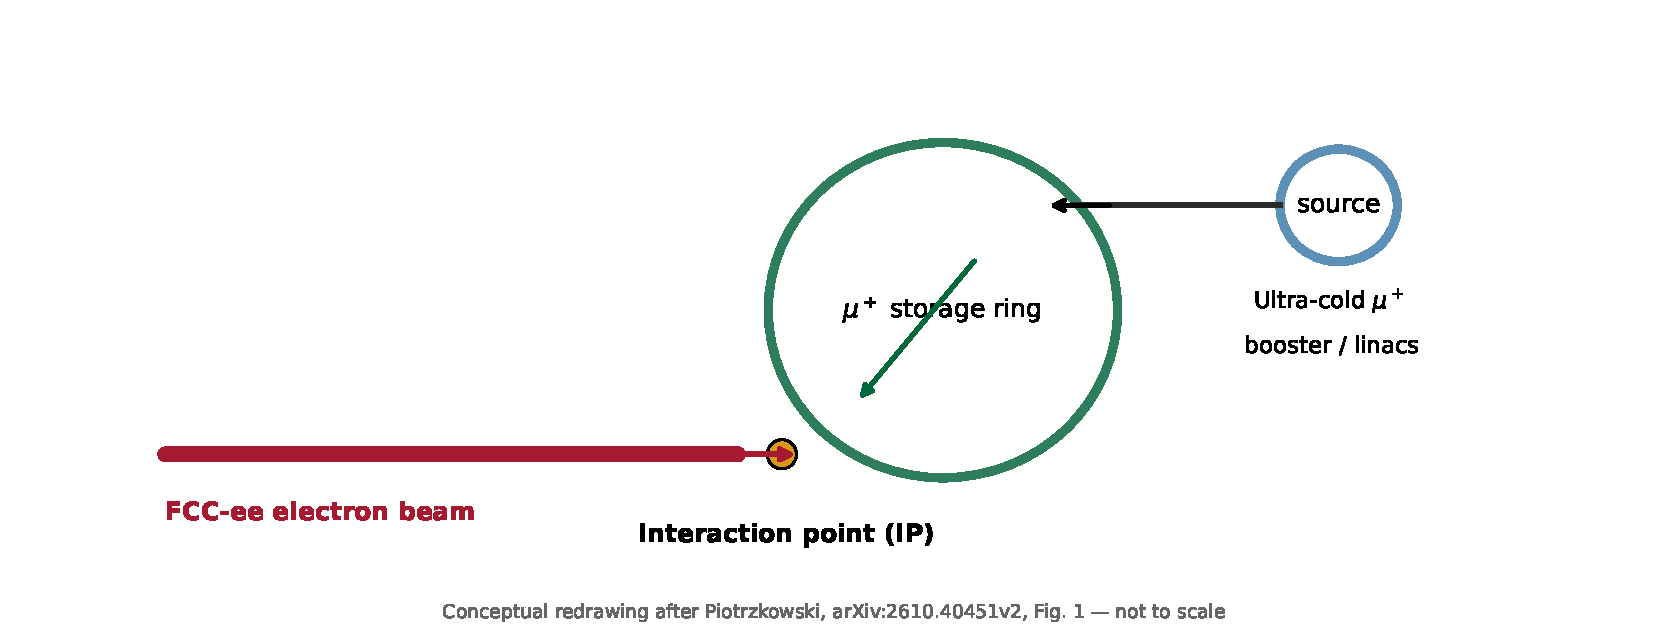
\includegraphics[width=\linewidth,height=0.47\textheight,keepaspectratio]{figures/Figure_FCCmue_concept_schematic.pdf}\end{center}
%\column{.39\textwidth}
%\begin{block}{Accelerator concept}
%\begin{itemize}
%\justifying
%\item Ultra-cold $\mu^+$ source and acceleration complex.
%\item Booster with two linacs; main $\mu^+$ storage ring.
%\item Head-on collision with FCC-ee electrons at shared IP.
%\item Concurrent and stand-alone options investigated.
%\end{itemize}\end{block}
%\end{columns}
%\key{A design proposal rather than a committed facility: machine and detector feasibility require further work.}

%\src{Concept schematic redrawn after Piotrzkowski, arXiv:2610.40451v2, Fig. 1, p. 3; not to scale.}
%\end{frame}





% Slide 6 / Beam Energies and Centre-of-Mass Reach
\begin{frame}[t]{Beam Energies and Centre-of-Mass Reach}
\small

\begin{center}\large
$\displaystyle s\simeq4E_{e^-}E_{\mu^+},\qquad \sqrt{s}\simeq 2\sqrt{E_{e^-}E_{\mu^+}}$
\end{center}
\begin{block}{Two distinct benchmark families}
\begin{center}\setlength{\tabcolsep}{6pt}
\begin{tabular}{llrrr}
\toprule
Family & Case & $E_{\mu^+}$ [GeV] & $E_{e^-}$ [GeV] & $\sqrt{s}$ [TeV]\\\midrule
FCC-$\mu e$ machine-like & low & 2000 & 120 & 0.9798\\
FCC-$\mu e$ machine-like & high & 5000 & 183 & 1.9131\\
Exact-energy scan & 1 TeV & 2000 & 125 & 1.0000\\
Exact-energy scan & 2 TeV & 5000 & 200 & 2.0000\\\bottomrule
\end{tabular}\end{center}
\end{block}
%\key{Do not mix the earlier 0.980/1.913 TeV $4b$ results with our exact 1/2 TeV inclusive scan.}

%\src{arXiv:2610.40451v2 (machine concept); 48-run CERN configuration JSON (exact points).}
\end{frame}





% Slide 7 / Luminosity, Staging and Running Assumptions
\begin{frame}[t]{Luminosity, Staging and Running Assumptions}
\footnotesize

\begin{block}{Revised proposal (arXiv v2), example 2 TeV $\mu^+$ beam}
\begin{center}\begin{tabular}{lcc}
\toprule
FCC-ee electron energy & 45.6 GeV & 120 GeV\\\midrule
$\sqrt{s}_{\mu e}$ & $\sim0.60$ TeV & $\sim0.98$ TeV\\
Estimated peak $\mathcal L$ [$10^{34}\,\mathrm{cm}^{-2}\mathrm{s}^{-1}$] & $4.5$ & $0.63$\\
Collision rate & 40 MHz & 1 MHz\\\bottomrule
\end{tabular}\end{center}
\end{block}
\begin{itemize}
\justifying
\item Values are \emph{proposal scenarios}, depending on source intensity, emittance and beam matching.
\item 2610.40451(v2) discusses multi-ab$^{-1}$ possibilities integrated over FCC-ee stages; distribution among energies and polarization settings is not fixed.
\item Stand-alone operation and the 5 TeV $\mu^+$ extension remain design options.
\end{itemize}
\key{Sensitivity estimates require $\mathcal L_{\rm int}$ at the exact energy and polarization; peak $\mathcal L$ is not integrated luminosity.}

%\src{Piotrzkowski, arXiv:2610.40451v2, Table 1, p. 5 and Sec. 4; v1 table differs.}
\end{frame}






% Slide 8 / FCC-ee and FCC-$\mu e$: Complementary Higgs Programmes
\begin{frame}[t]{FCC-ee and FCC-$\mu e$: Complementary Higgs Programmes}
\small

\begin{columns}%%%[T,onlytextwidth]
\column{.48\textwidth}
\begin{exampleblock}{FCC-ee: precision factory}
\begin{itemize}
\justifying
\item $e^+e^-$ at $\sqrt{s}\simeq240$ and 365 GeV.
\item $ZH$ recoil method, Higgs couplings/width.
\item Precision $HZZ$, $HWW$, heavy-flavour decays.
\item Indirect self-coupling information through radiative corrections.
\end{itemize}\end{exampleblock}
\column{.49\textwidth}
\begin{alertblock}{FCC-$\mu e$: high-energy complement}
\begin{itemize}
\justifying
\item $WW/ZZ$-fusion $H$ and $HH$ at $\sim1$--2 TeV.
\item Direct tree-level $HH$ dependence on $\lambda_3$.
\item Polarization and $HHVV$ information.
\item Potential combined Higgs-coupling / EFT interpretation.
\end{itemize}\end{alertblock}
\end{columns}

%\key{Best physics case is \emph{combined information}, not unsupported claims that either machine supersedes the other.}

%\src{FCC Feasibility Study, EPJC 85 (2025) 1468; Piotrzkowski arXiv:2610.40451v2.}
\end{frame}






% Slide 9 / Detector Challenges from Highly Asymmetric Beams
\begin{frame}[t]{Detector Challenges from Highly Asymmetric Beams}
\small

\begin{columns}%%%[T,onlytextwidth]
\column{0.55\textwidth}
\begin{block}{Kinematic acceptance}
\begin{itemize}
\justifying
\item Large laboratory-frame boost along the energetic $\mu^+$ beam.
\item Forward charged leptons in NC production.
\item Missing momentum for CC channels.
\item $4b$ tagging in extended $\eta$ acceptance.
\end{itemize}\end{block}
\column{0.55\textwidth}
\begin{block}{Machine-detector interface}
\begin{itemize}
\justifying
\item Decay positrons from stored $\mu^+$ beam.
\item Nozzle shielding and beam separation.
\item Trigger, calibration and backgrounds.
\item Practical polarized-beam luminosity.
\end{itemize}\end{block}
\end{columns}

\key{Generator cuts of $|\eta_b|<5$ are not a detector design; reconstructible final states require dedicated simulation.}

%\src{Piotrzkowski arXiv:2610.40451v2, Sec. 3; detector topics are future studies.}
\end{frame}




\part{Calculations and definitions}
\section{Calculations and definitions}





% Slide 10 / Complete Inventory of Investigated Higgs Processes
\begin{frame}[t]{Complete Inventory of Investigated Higgs Processes}
\small

\begin{columns}%%%[T,onlytextwidth]
\column{0.5\textwidth}
\begin{exampleblock}{FCC-$\mu e$ completed}
\begin{itemize}\item CC: $\nu_e\bar\nu_\mu H$, $\nu_e\bar\nu_\mu HH$.
\item NC: $e^-\mu^+H$, $e^-\mu^+HH$.
\item Resonant $HH\to4b$ and full $\nu\bar\nu4b$.
\item NC $HH\to4b$, $b\bar b H\to4b$, full NC $4b$ and continuum diagnostic.
\end{itemize}\end{exampleblock}
\column{0.5\textwidth}
\begin{alertblock}{$\mu^+\mu^-$ comparison completed}
\begin{itemize}\item CC $HH\to4b$; full $\nu\bar\nu4b$.
\item NC associated $b\bar bH$.
\item Resonant $ZH\to4b$ at 1,2 TeV.
\end{itemize}\end{alertblock}
\begin{block}{Not yet calculated}
$\mu^+e^-\to\nu_e\bar\nu_\mu HHH$ and $\mu^+e^-\to\mu^+e^-HHH$, anomalous-coupling scans.
\end{block}
\end{columns}

%\src{CERN result archives October--November 2026; proposed channels flagged separately.}
\end{frame}





% Slide 11 / CERN MadGraph Workflow and Reproducibility
\begin{frame}[t]{MadGraph Workflow and Reproducibility}
\footnotesize

\begin{center}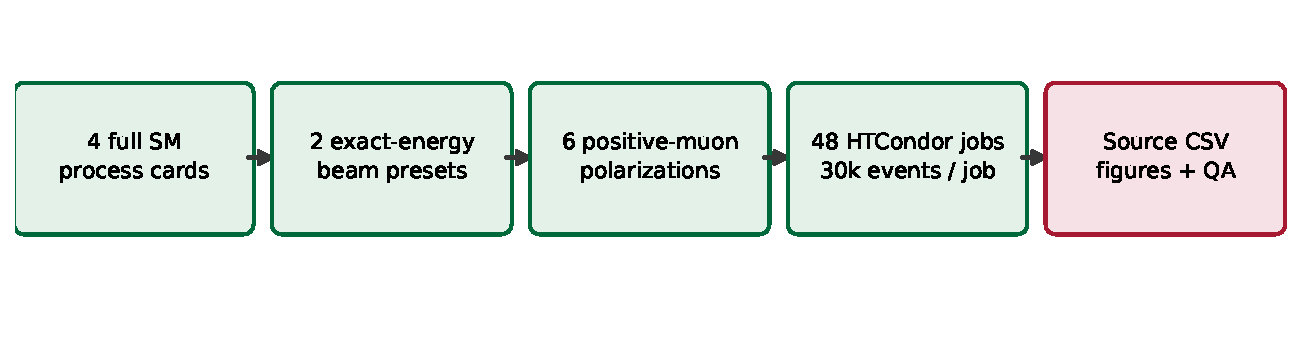
\includegraphics[width=\linewidth,height=0.450\textheight,keepaspectratio]{figures/Figure_scan_workflow.pdf}
\end{center}

\begin{columns}%%%[T,onlytextwidth]
\column{0.5\textwidth}
\begin{block}{Production}
\begin{itemize}
\justifying 
\item MadGraph5\_aMC@NLO 3.6.4, LO SM.
\item Original process and parameter cards preserved.
\item 48 exact-energy HTCondor jobs on CERN.
\item 30,000 event requests per job; individual seeds.
\end{itemize}\end{block}
\column{0.5\textwidth}
\begin{block}{Quality status}
\begin{itemize}
\justifying
\item 48/48 returned result records.
\item Beam polarizations and energies audited.
\item MC integration errors available.
\item \textbf{Still needed:} independent seeds; forward NC stability.
\end{itemize}\end{block}
\end{columns}

%\src{CERN 48-run review ZIP, run cards, quality\_checks.json; status COMPLETED\_UNVALIDATED.}
\end{frame}









% Slide 12 / Inclusive, Decayed and Fiducial Cross Sections
\begin{frame}[t]{Inclusive, Decayed and Fiducial Cross Sections}
\small

\begin{center}\setlength{\tabcolsep}{5pt}
\begin{tabular}{p{2.8cm}p{4.0cm}p{4.4cm}}\toprule
Dataset & Process definition & Selection / normalization\\\midrule
Inclusive $H/HH$ & Stable $H$, full CC/NC LO matrix & No generation kinematic cuts; output $\sigma_{\rm prod}$\\
Resonant $HH\to4b$ & Two $H\to b\bar b$ decays & $|\eta_b|<5$; two 110--130 GeV pairs\\
NC $4b$ & NC charged leptons & Above $b$ cuts; $p_{T,\ell}>1$ GeV at generation\\
Muon $ZH\to4b$ & Explicit $Z,H\to b\bar b$ & $|\eta_b|<5$; two 80--130 GeV pairs\\\bottomrule
\end{tabular}\end{center}

%\key{Do not compare stable-H inclusive rates directly with fiducial four-bottom rates without the decay, cut and EW input conventions.}

%\src{48-run dataset; Oct. 2026 CC/NC reports; ZH report 29 Oct. 2026.}
\end{frame}








% Slide 13 / Polarization, Electroweak Inputs and Branching Fractions
\begin{frame}[t]{Polarization, Electroweak Inputs and Branching Fractions}
\small

\begin{columns}%%%[T,onlytextwidth]
\column{0.50\textwidth}
\begin{block}{Inclusive scan conventions}
\begin{itemize}\item MG5 beam 1: $e^-$, $P_{e^-}=0$.
\item MG5 beam 2: $\mu^+$; $P_{\mu^+}=0\ldots100\%$.
\item Right-helicity $\mu^+$ contributes to CC.
\item Two separate exact-energy beam cards.
\end{itemize}
\end{block}
\column{0.50\textwidth}
\begin{alertblock}{Historical $4b$ normalization}
\begin{itemize}\item Earlier resonant $HH\to4b$ packages used
$\mathrm{BR}(H\to b\bar b)=0.844640$.
\item Precision-SM nominal value is $\sim0.58$.
\item Ratios/absolute $4b$ yields are not interchangeable before reweighting or regeneration.
\end{itemize}\end{alertblock}
\end{columns}

%\key{Check original parameter cards, resonance treatment, and branching fractions before quantitative sensitivity fits.}

%\src{CERN proc/run/param cards; NC three-process audit; CC 1 TeV polarization audit.}
\end{frame}


\part{Inclusive H/HH and polarization}
\section{Inclusive H/HH and polarization}


% Slide 14 / Four Full-Matrix-Element Inclusive Higgs Channels
\begin{frame}[t]{Four Full-Matrix-Element Inclusive Higgs Channels}
\small

\begin{center}\setlength{\tabcolsep}{5pt}
\begin{tabular}{lp{8.4cm}}\toprule
Channel & MadGraph5 generation command\\\midrule
CC $H$ & \texttt{generate e- mu+ > ve vm\textasciitilde{} h QCD=0}\\[.25em]
CC $HH$ & \texttt{generate e- mu+ > ve vm\textasciitilde{} h h QCD=0}\\[.25em]
NC $H$ & \texttt{generate e- mu+ > e- mu+ h QCD=0}\\[.25em]
NC $HH$ & \texttt{generate e- mu+ > e- mu+ h h QCD=0}\\\bottomrule
\end{tabular}\end{center}
\begin{block}{Physics content}
Full tree-level SM amplitudes without diagram exclusions; stable Higgs bosons; $WW/ZZ$ fusion topology. $HH$ includes $HHVV$, separate $HVV$, and $H^*\to HH$ contributions.
\end{block}

\key{CC and NC probe complementary initial-state chiral currents and Higgs-gauge couplings.}

%\src{Original 48-run MadGraph process-card exports.}
\end{frame}







% Slide 15 / Single-Higgs Production: Original MadGraph Diagrams
\begin{frame}[t]{Single-Higgs Production: Original MadGraph Diagrams}
\small

\begin{columns}%%%[T,onlytextwidth]
\column{0.5\textwidth}
\centering\textbf{CC: $\mu^+e^-\to\bar\nu_\mu\nu_eH$}\\[.2em]
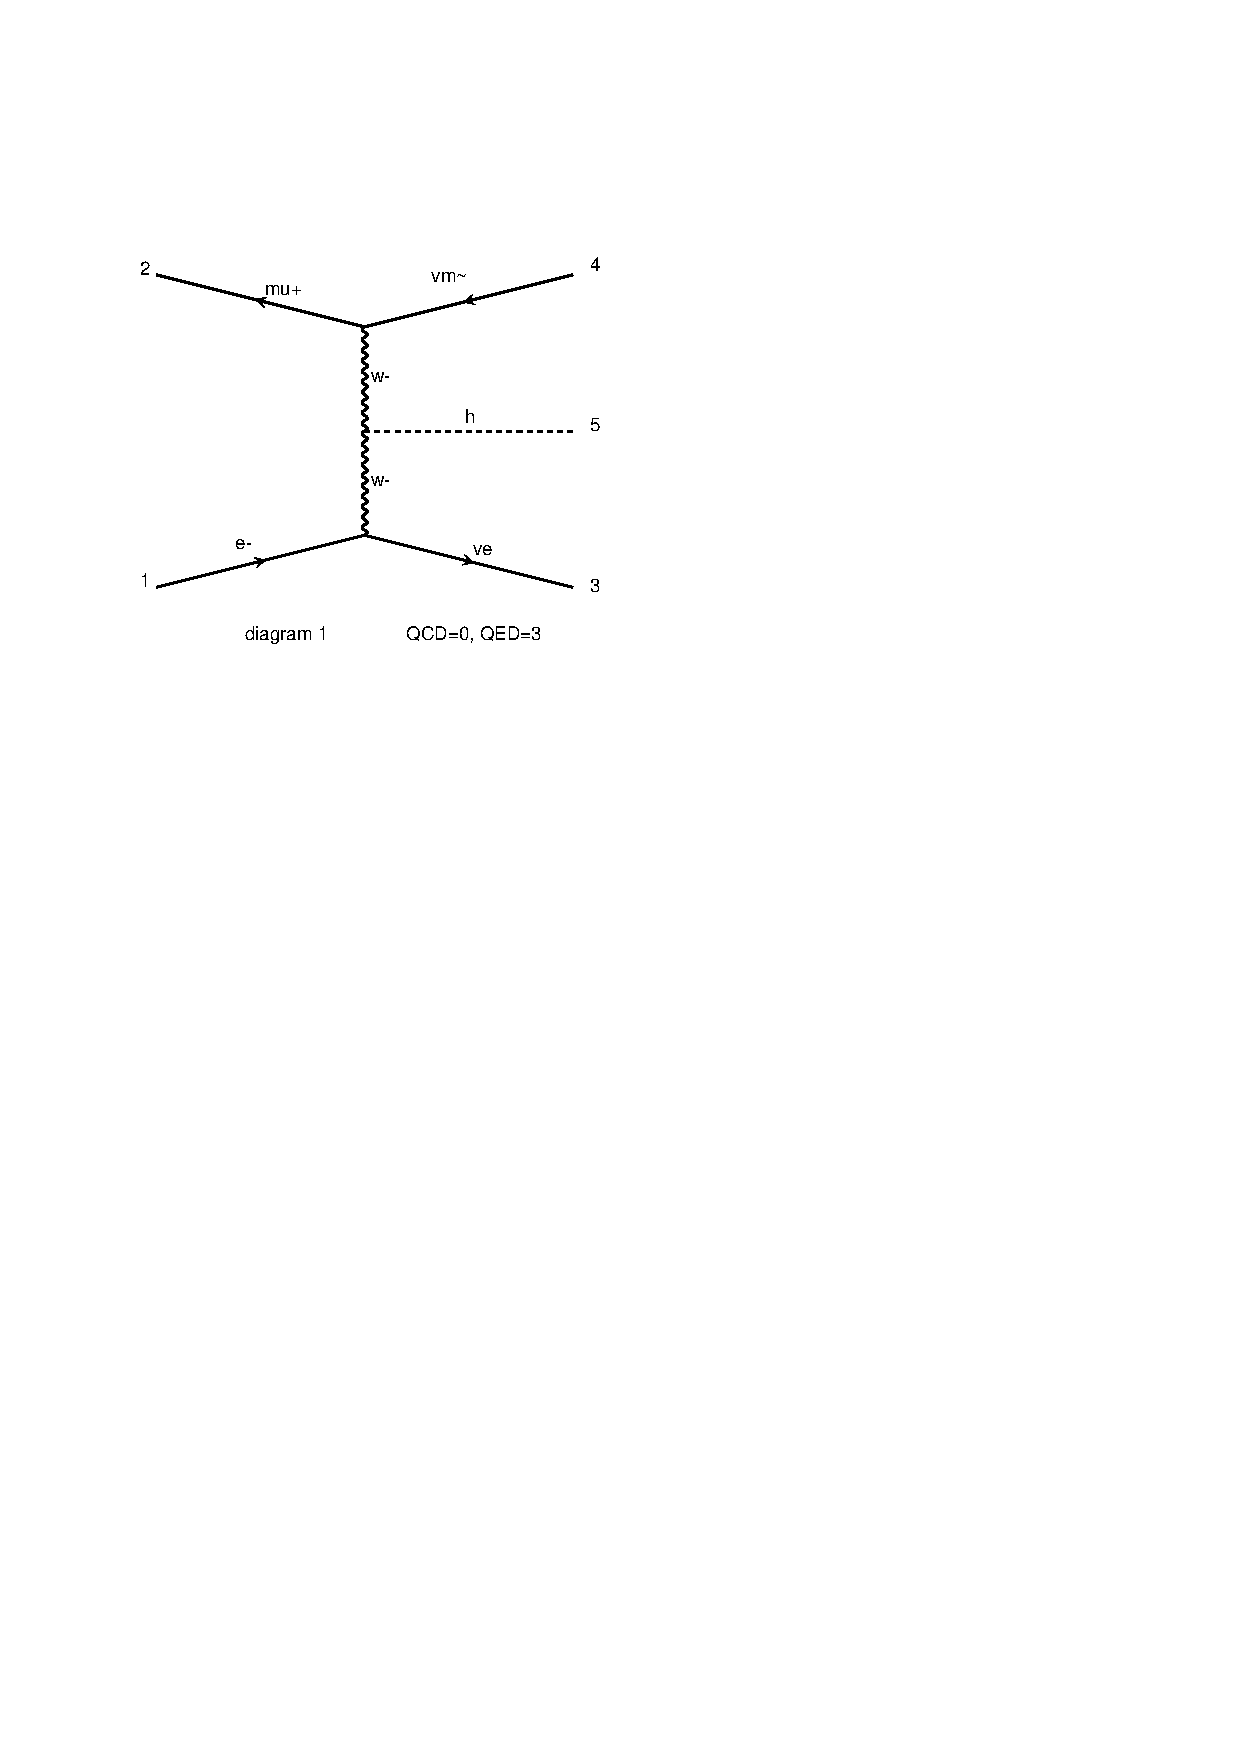
\includegraphics[width=0.98\linewidth,height=0.55\textheight,keepaspectratio]{figures/CC_H_diagrams_cropped.pdf}\\[.3em]
{\scriptsize One exported diagram; $HWW$ fusion coupling.}
\column{.49\textwidth}
\centering\textbf{NC: $\mu^+e^-\to\mu^+e^-H$}\\[.2em]
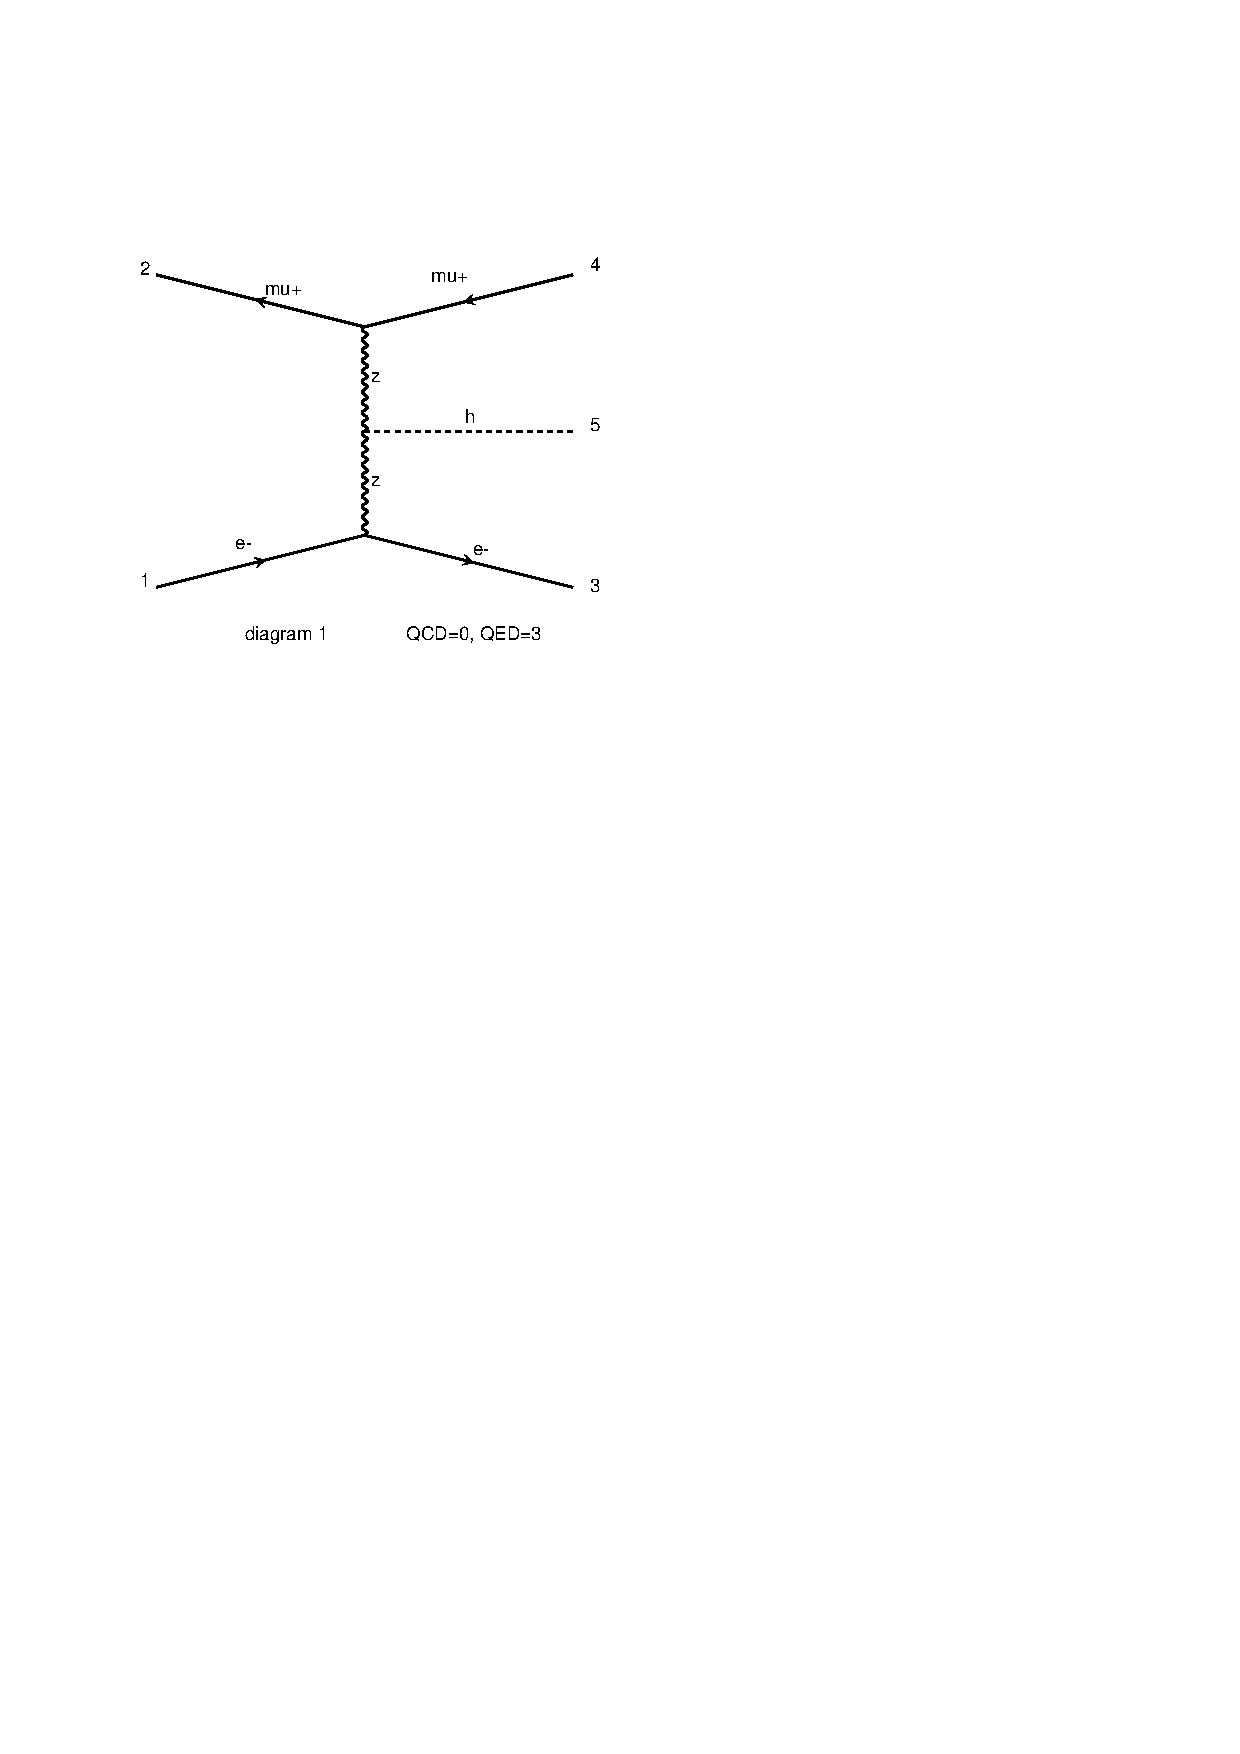
\includegraphics[width=0.98\linewidth,height=0.5\textheight,keepaspectratio]{figures/NC_H_diagrams_cropped.pdf}\\[.3em]
{\scriptsize One exported diagram; $HZZ$ fusion coupling.}
\end{columns}
\key{These are \emph{original exported MadGraph diagrams}.}

%\src{CERN MG5 original CC\_H/matrix.pdf and NC\_H/matrix.pdf (vector diagrams).}
\end{frame}







% Slide 16 / CC Double Higgs: Four Original MadGraph Diagrams
\begin{frame}[t]{CC Double Higgs: Four Original MadGraph Diagrams}
\footnotesize

\begin{columns}%%%[T,onlytextwidth]
\column{0.65\textwidth}
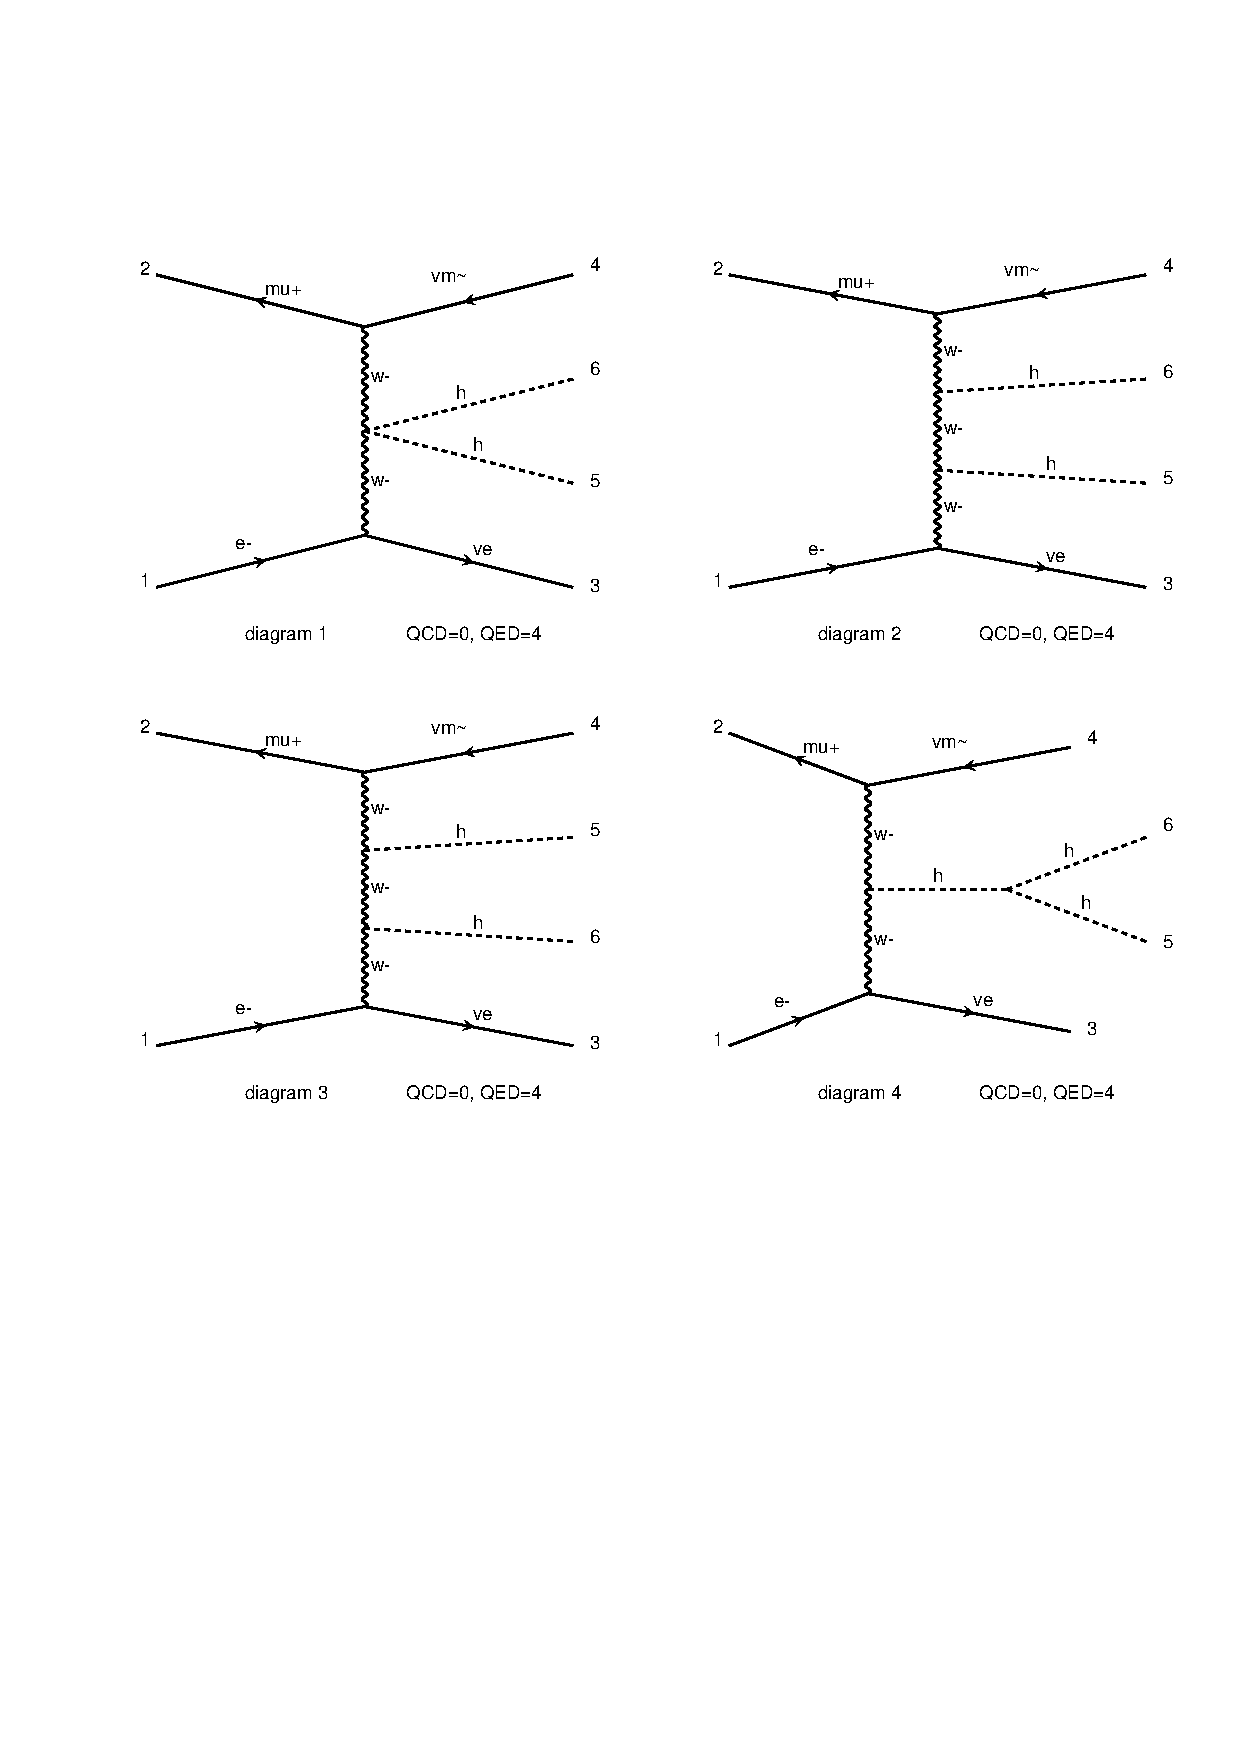
\includegraphics[width=\linewidth,height=0.65\textheight,keepaspectratio]{figures/CC_HH_diagrams_cropped.pdf}
\column{0.45\textwidth}
\begin{block}{Diagram identification}
\begin{itemize}
\justifying 
\item \textbf{1:} $HHWW$ contact.
\item \textbf{2,3:} separate Higgs emissions through $HWW$ couplings.
\item \textbf{4:} $W^*W^*\to H^*\to HH$; trilinear $HHH$ coupling.
\end{itemize}\end{block}
\end{columns}
\key{The unrestricted CC $HH$ process includes all four tree diagrams and their interference.}

%\src{Original CERN MG5 CC\_HH/matrix.pdf; diagram IDs checked against original export.}
\end{frame}





% Slide 17 / NC Double Higgs: Four Original MadGraph Diagrams
\begin{frame}[t]{NC Double Higgs: Four Original MadGraph Diagrams}
\footnotesize

\begin{columns}%%%[T,onlytextwidth]
\column{.64\textwidth}
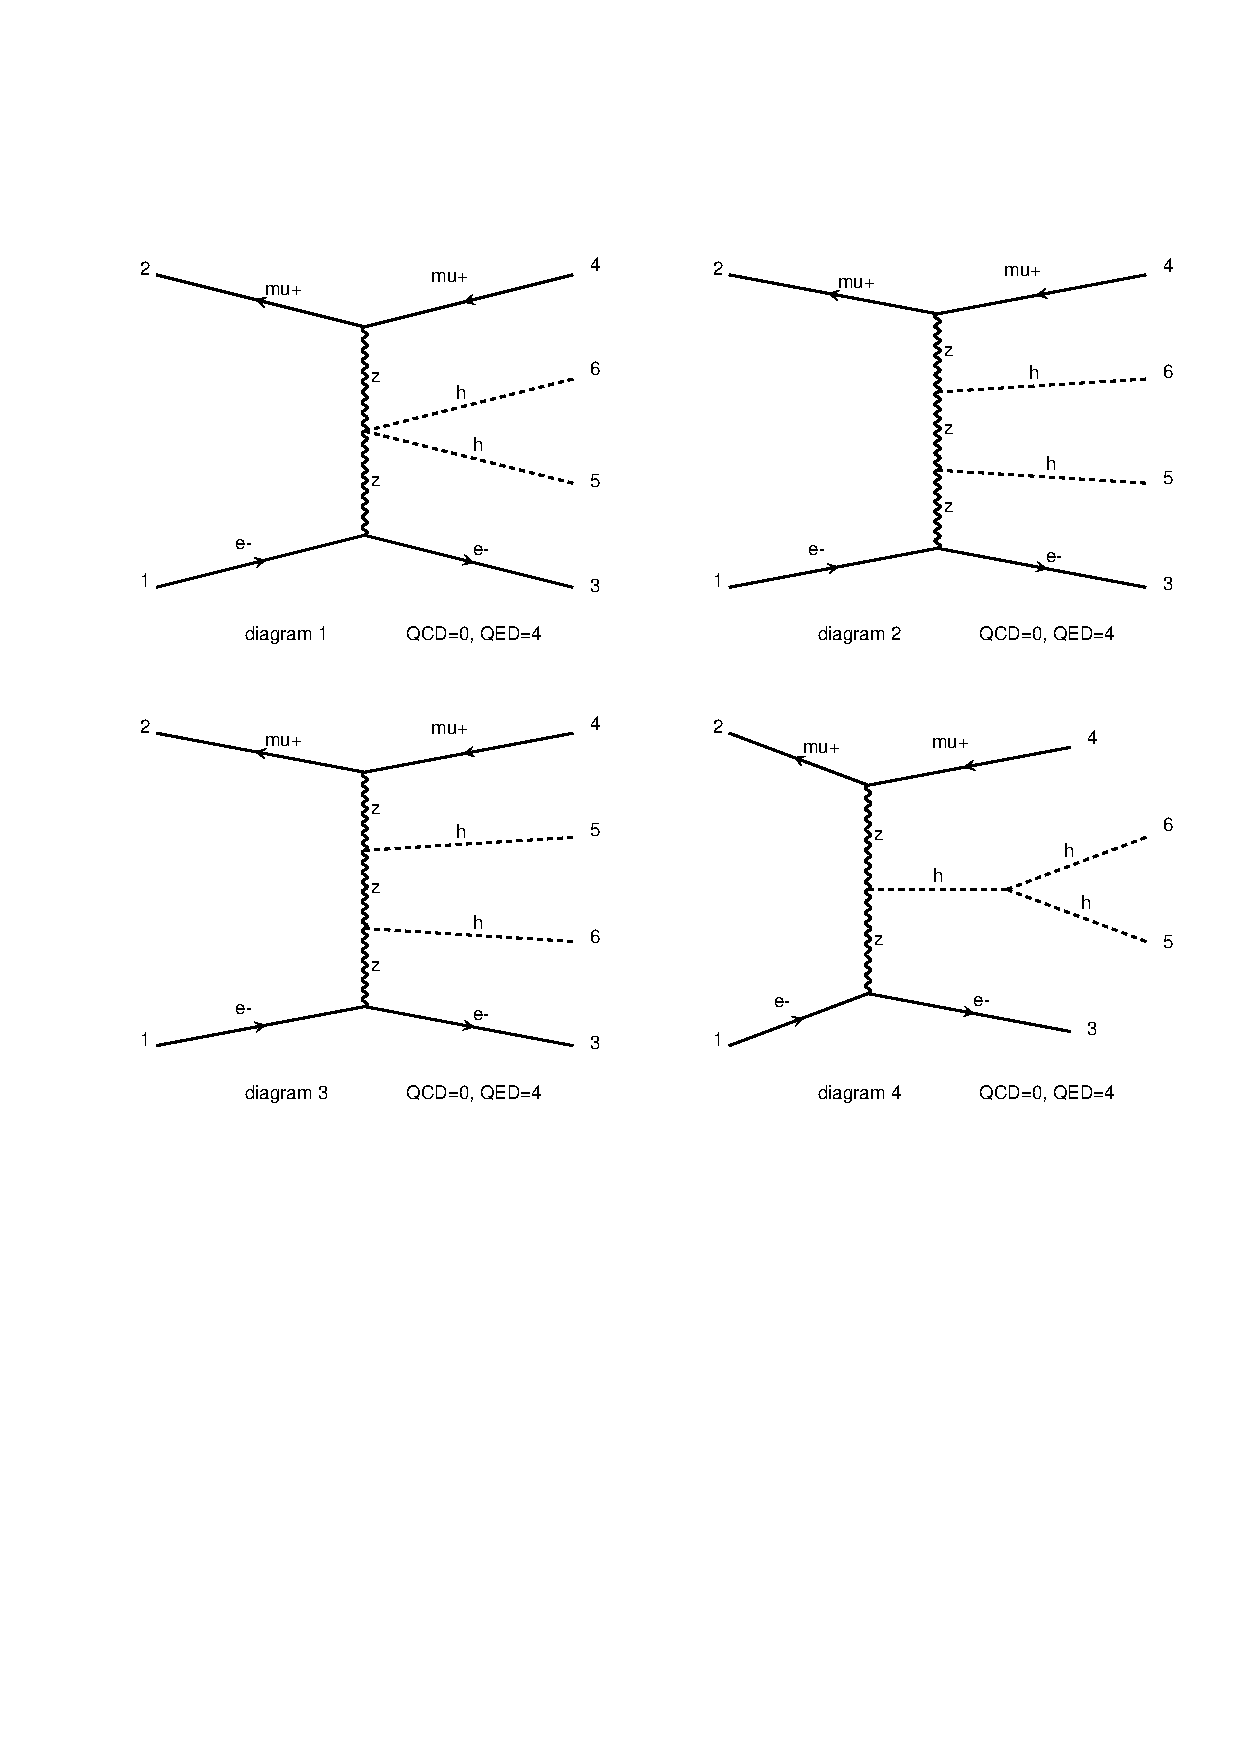
\includegraphics[width=\linewidth,height=0.65\textheight,keepaspectratio]{figures/NC_HH_diagrams_cropped.pdf}
\column{0.45\textwidth}
\begin{block}{Diagram identification}
\begin{itemize}
\justifying 
\item \textbf{1:} $HHZZ$ contact.
\item \textbf{2,3:} separate Higgs emissions through $HZZ$ couplings.
\item \textbf{4:} $Z^*Z^*\to H^*\to HH$; trilinear $HHH$ coupling.
\end{itemize}\end{block}
\end{columns}
\key{The neutral-current amplitude includes contact, sequential and virtual-Higgs contributions coherently.}

%\src{Original CERN MG5 NC\_HH/matrix.pdf; diagram IDs checked against export.}
\end{frame}






% Slide 18 / Krzysztof's Question: Are All HH Contributions Included?
\begin{frame}[t]{Krzysztof's Question: Are All HH Contributions Included?}
\footnotesize

\begin{alertblock}{Question addressed}
\justifying 
Are both the Higgs self-coupling diagram $H^*\to HH$ and the separate $HVV$-emission graphs included?
\end{alertblock}
\begin{center}\large
$\displaystyle \mathcal M_{HH}=\mathcal M_{HHVV}+\mathcal M_{\mathrm{separate}\,HVV}+\mathcal M_{\lambda_3}$\\[.15em]
$\displaystyle\sigma_{HH}\propto\bigl|\mathcal M_{HH}\bigr|^2$
\end{center}
\begin{itemize}
\justifying 
\item \textbf{Yes:} original CC/NC MG5 exports contain diagrams 1-4, including virtual $H^*$ exchange.
\item Amplitude-level interference is retained; no diagram-specific cross sections were calculated.
\item Arbitrary subsets of gauge-related diagrams need not be independently gauge invariant.
\end{itemize}
\key{The existing SM baselines contain $\lambda_3$; a coupling scan is needed to quantify sensitivity.}

%\src{Original CC\_HH and NC\_HH MadGraph diagrams; process\_card QCD=0.}
\end{frame}





% Slide 19 / Richard's Six-Point Polarization Task: 48 CERN Runs
\begin{frame}[t]{Richard's Six-Point Polarization Task: 48 MG Runs}
\footnotesize

\begin{center}\LARGE\color{FCCgreen}\bfseries $4\times2\times6=48$\, production configurations\end{center}

\begin{center}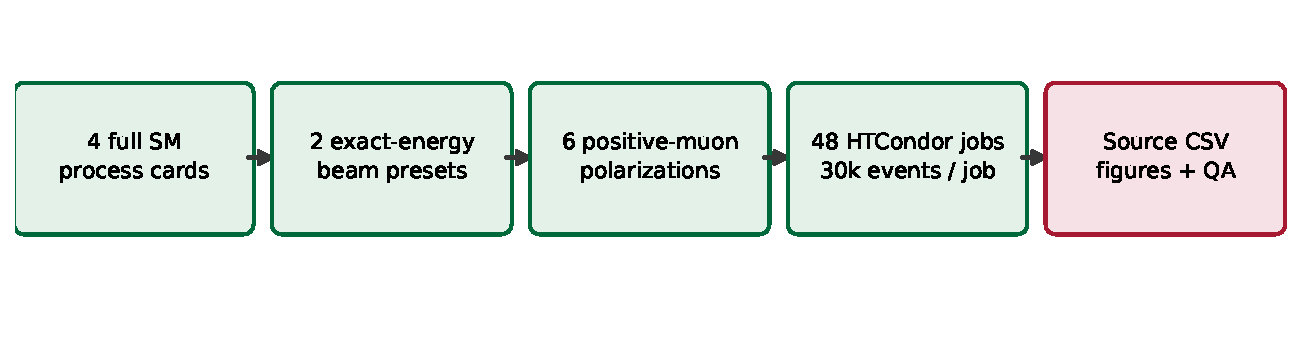
\includegraphics[width=\linewidth,height=0.45\textheight,keepaspectratio]{figures/Figure_scan_workflow.pdf}
\end{center}


\begin{columns}%%%[T,onlytextwidth]
\column{0.5\textwidth}
\begin{block}{Input scan}
\begin{itemize}\item 4 channels: CC/NC $H$, $HH$.
\item Exact $\sqrt{s}=1,2$ TeV.
\item $P_{\mu^+}=0,20,40,60,80,100\%$.
\end{itemize}\end{block}
\column{0.5\textwidth}
\begin{block}{CERN output}
\begin{itemize}\item 30,000 events per configuration.
\item 48/48 archived cross-section records.
\item Run-card and polarity QA passed; physics convergence ongoing.
\end{itemize}\end{block}
\end{columns}

%\src{48-job full/exact CERN review archive; November 2026.}
\end{frame}







% Slide 20 / Inclusive Higgs Cross Sections at 1 TeV
\begin{frame}[t]{Inclusive Higgs Cross Sections at 1 TeV}
\scriptsize

\begin{block}{Exact $\sqrt{s}=1$ TeV; $e^-(125)$ GeV $+\,\mu^+(2000)$ GeV; $P_{e^-}=0$}
\scriptsize\centering Each entry: $\sigma\pm\delta\sigma_{\rm MC}$ [fb].\\[-.6em]
\begin{center}\setlength{\tabcolsep}{3pt}\renewcommand{\arraystretch}{1.23}\begin{tabular}{rllll}\toprule $P_{\mu^+}$ & CC $H$ & CC $HH$ & NC $H$ & NC $HH$ \\ \midrule
0\% & $210.540\pm0.209$ & $0.074384\pm0.00013$ & $20.835\pm0.025$ & $0.0096201\pm0.0000146$ \\
20\% & $252.710\pm0.158$ & $0.088979\pm0.00015$ & $21.770\pm0.015$ & $0.010045\pm0.0000167$ \\
40\% & $294.730\pm0.271$ & $0.104016\pm0.00019$ & $22.660\pm0.014$ & $0.010487\pm0.0000160$ \\
60\% & $336.830\pm0.199$ & $0.118825\pm0.00021$ & $23.611\pm0.019$ & $0.010895\pm0.0000148$ \\
80\% & $378.570\pm0.243$ & $0.133230\pm0.00023$ & $24.476\pm0.015$ & $0.011308\pm0.0000174$ \\
100\% & $421.150\pm0.433$ & $0.148239\pm0.00024$ & $25.402\pm0.018$ & $0.011723\pm0.0000180$ \\
\bottomrule\end{tabular}\end{center}
\end{block}
\key{At $P_{\mu^+}=80\%$: CC $HH=0.13323$ fb and NC $HH=0.011308$ fb; stable Higgs, not $4b$.}

%\src{CERN original cross\_sections.csv; error from generator integration (not detector/theory).}
\end{frame}







% Slide 21 / Inclusive Higgs Cross Sections at 2 TeV
\begin{frame}[t]{Inclusive Higgs Cross Sections at 2 TeV}
\scriptsize

\begin{block}{Exact $\sqrt{s}=2$ TeV; $e^-(200)$ GeV $+\,\mu^+(5000)$ GeV; $P_{e^-}=0$}
\scriptsize\centering Each entry: $\sigma\pm\delta\sigma_{\rm MC}$ [fb].\\[-.6em]
\begin{center}\setlength{\tabcolsep}{3pt}\renewcommand{\arraystretch}{1.23}\begin{tabular}{rllll}\toprule $P_{\mu^+}$ & CC $H$ & CC $HH$ & NC $H$ & NC $HH$ \\ \midrule
0\% & $386.010\pm0.303$ & $0.418510\pm0.00066$ & $38.991\pm0.030$ & $0.054712\pm0.0000851$ \\
20\% & $463.490\pm0.399$ & $0.502952\pm0.00085$ & $40.760\pm0.027$ & $0.057089\pm0.0000871$ \\
40\% & $540.620\pm0.371$ & $0.587089\pm0.00100$ & $42.460\pm0.045$ & $0.059636\pm0.0000859$ \\
60\% & $617.270\pm0.428$ & $0.671917\pm0.00115$ & $44.171\pm0.042$ & $0.062066\pm0.0000868$ \\
80\% & $695.000\pm0.614$ & $0.754495\pm0.00128$ & $45.829\pm0.055$ & $0.064299\pm0.0000957$ \\
100\% & $772.690\pm0.517$ & $0.839521\pm0.00140$ & $47.642\pm0.033$ & $0.066770\pm0.00010$ \\
\bottomrule\end{tabular}\end{center}
\end{block}
\key{CC $HH$: 0.41851 (P0) $\to$ 0.75450 (P80) $\to$ 0.83952 fb (P100).}

%\src{CERN original cross\_sections.csv; exact-energy scan (not earlier 1.913 TeV study).}
\end{frame}








% Slide 22 / Absolute Higgs Cross Sections versus Muon Polarization
\begin{frame}[t]{Absolute Higgs Cross Sections versus Muon Polarization}
\scriptsize

\begin{center}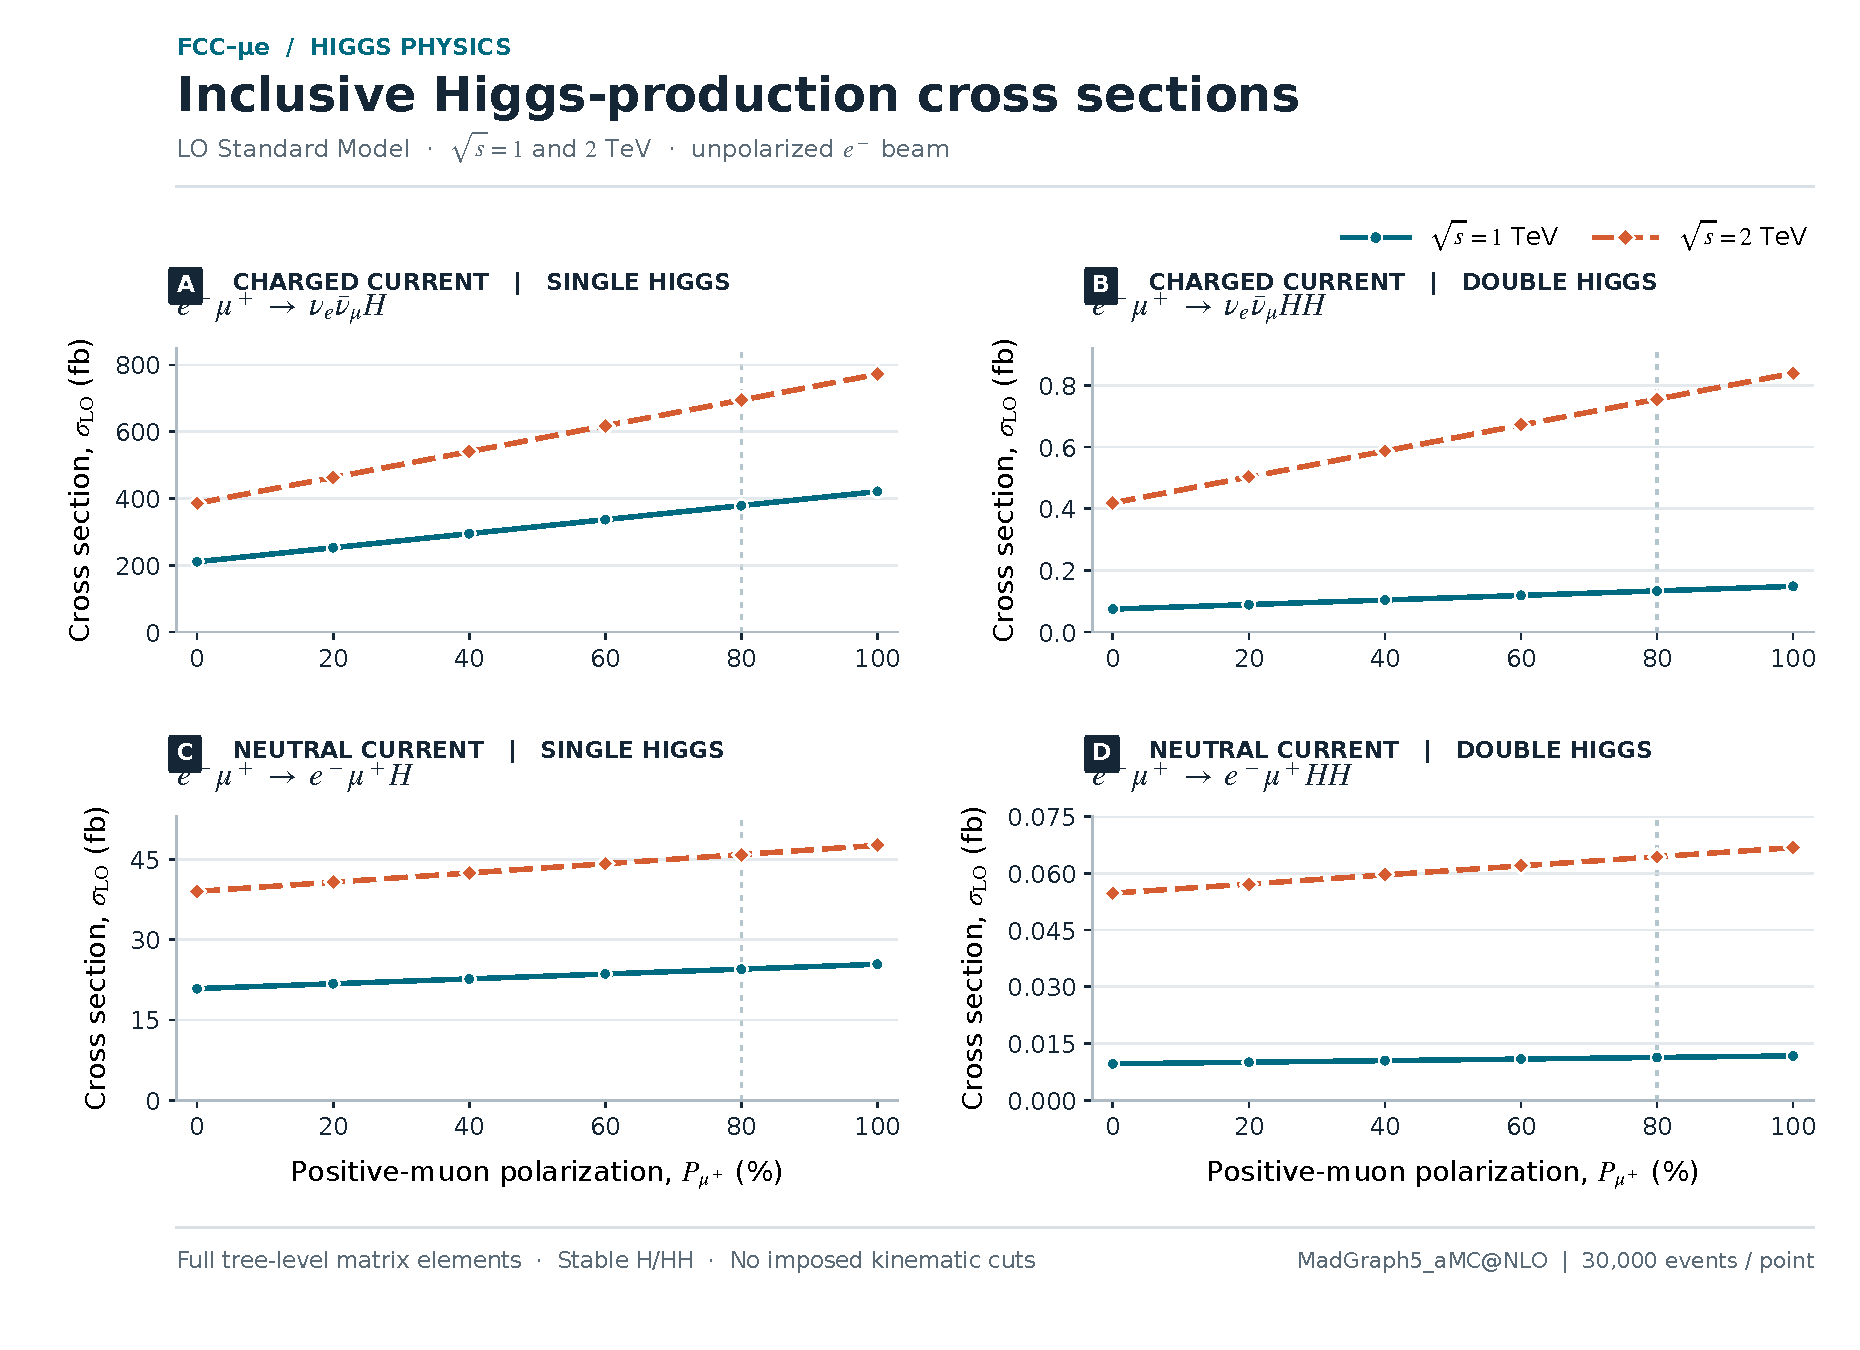
\includegraphics[width=\linewidth,height=0.65\textheight,keepaspectratio]{figures/Figure_1_absolute_cross_sections.pdf}\end{center}
\vspace{-1em}\key{CC rates are larger; the higher energy strongly benefits the $HH$ channel. Error bars are MC integration errors.}

%\src{Regenerated vector plot from 48 original CERN scan rows; stable H, no cuts.}
\end{frame}







% Slide 23 / Polarization Enhancement Ratios: CC versus NC
\begin{frame}[t]{Polarization Enhancement Ratios: CC versus NC}
\scriptsize

\begin{center}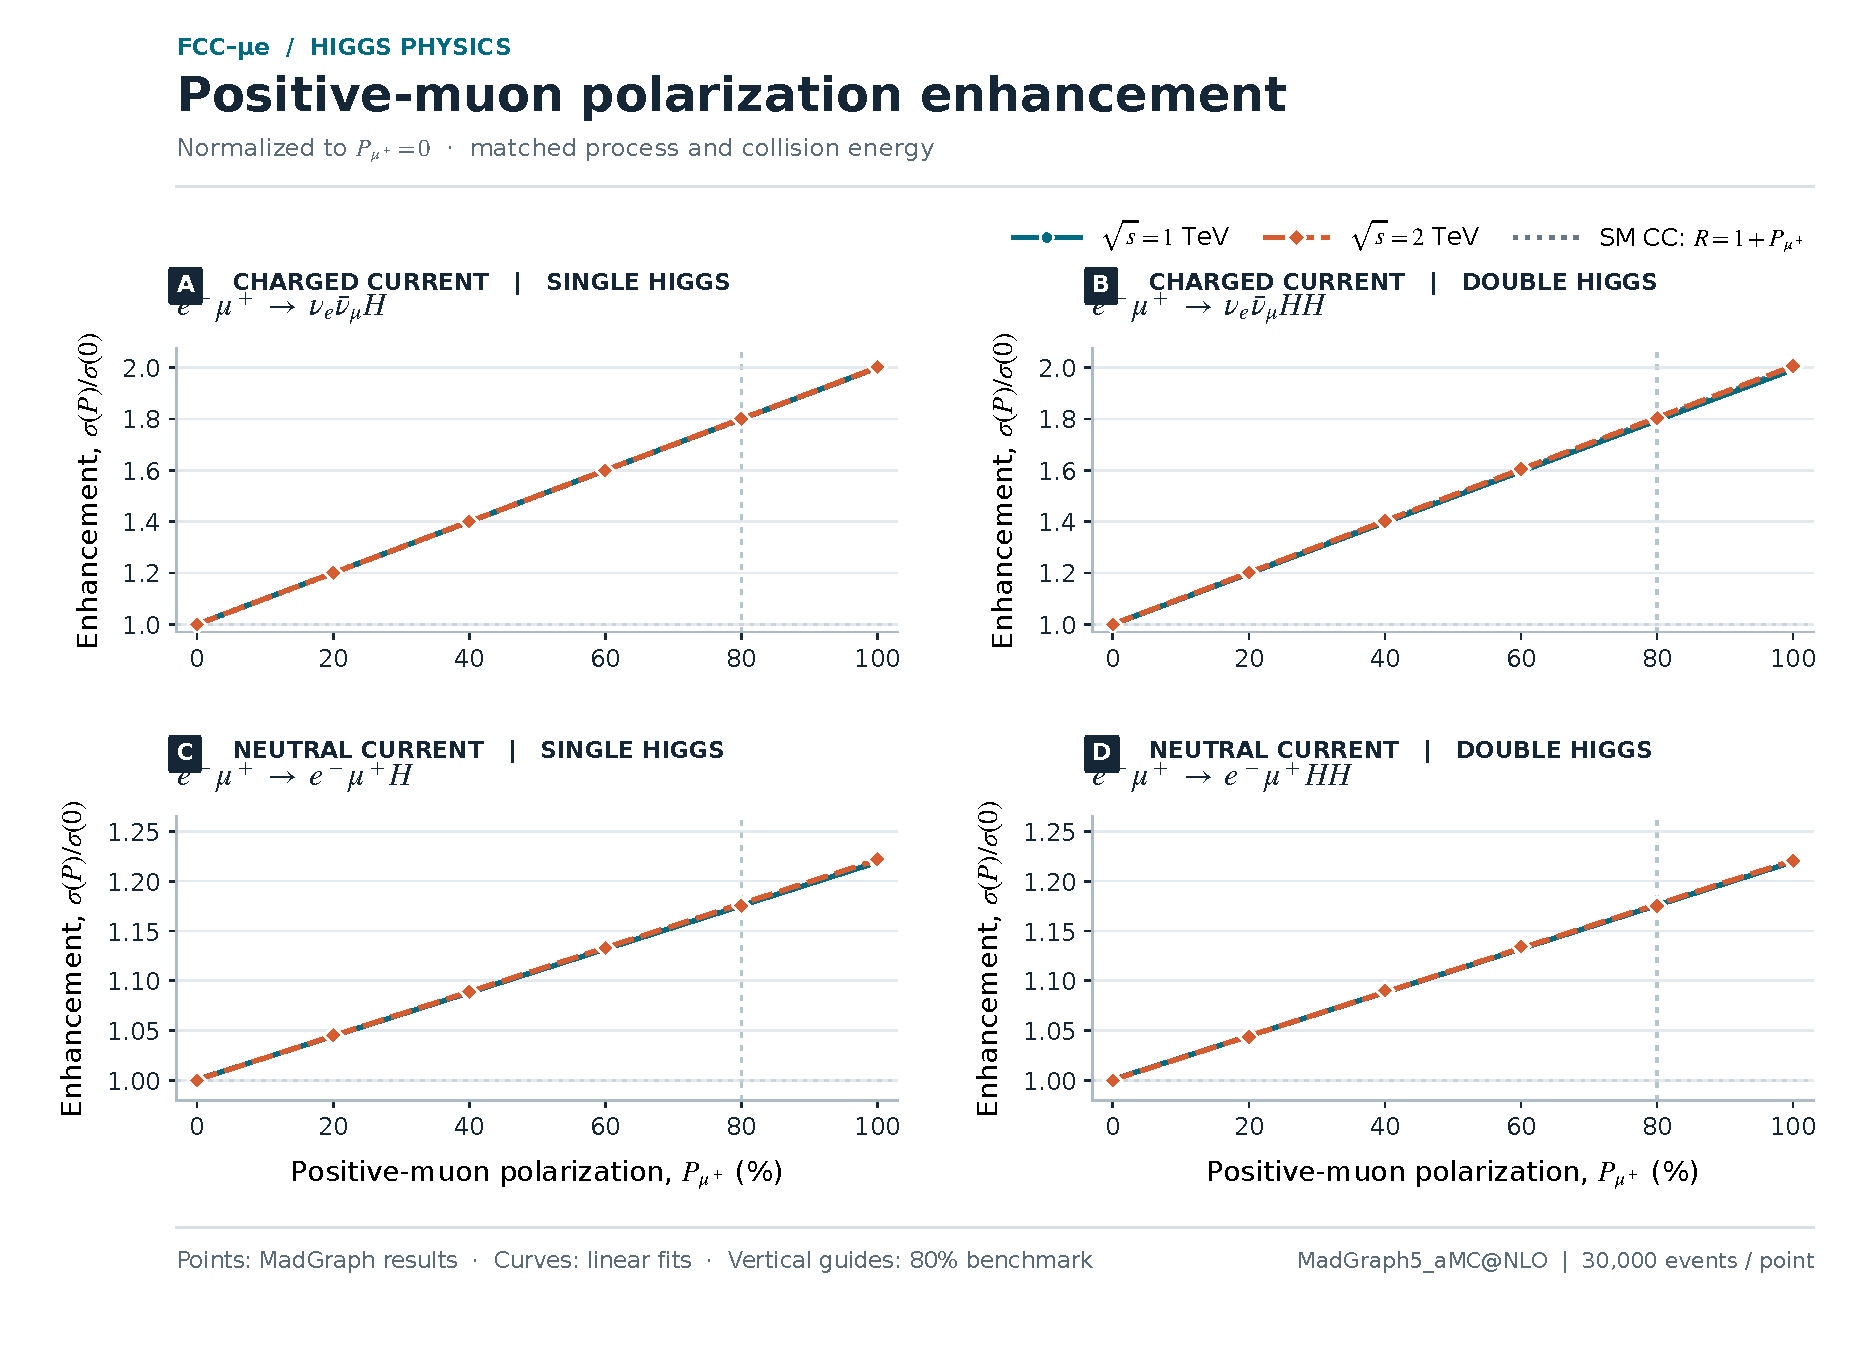
\includegraphics[width=\linewidth,height=0.65\textheight,keepaspectratio]{figures/Figure_2_polarization_ratios.pdf}\end{center}
\vspace{-1em}\key{$R_{CC}(80\%)\simeq1.8$, while $R_{NC}(80\%)\simeq1.175$ for both $H$ and $HH$.}

%\src{Original-data vector plot; denominator is the unpolarized rate for same process and energy.}
\end{frame}

% Slide 24 / Polarization Slopes and Linearity Tests
\begin{frame}[t]{Polarization Slopes and Linearity Tests}
\small

\begin{center}\normalsize $\sigma(p)=a(1+Ap),\qquad p=P_{\mu^+}/100$\end{center}
\begin{center}\setlength{\tabcolsep}{5pt}\renewcommand{\arraystretch}{1.15}
\begin{tabular}{lccrr}\toprule
 & $A(1\ \mathrm{TeV})$ & $A(2\ \mathrm{TeV})$ & $\chi^2/4$ (1 TeV) & $\chi^2/4$ (2 TeV)\\\midrule
CC $H$ & $0.9982\pm0.0020$ & $1.0007\pm0.0018$ & 1.77/4 & 2.38/4\\
CC $HH$ & $0.9934\pm0.0040$ & $1.0053\pm0.0039$ & 2.84/4 & 0.94/4\\
NC $H$ & $0.2181\pm0.0012$ & $0.2208\pm0.0011$ & 5.08/4 & 3.40/4\\
NC $HH$ & $0.2186\pm0.0022$ & $0.2204\pm0.0022$ & 1.93/4 & 3.36/4\\\bottomrule
\end{tabular}\end{center}
\begin{exampleblock}{Interpretation}
$A_{CC}\simeq1$ (chiral charged weak current); $A_{NC}\simeq0.22$ (parity-violating $Z$ couplings). Fits test generator behavior, not Higgs-coupling measurement precision.
\end{exampleblock}

%\src{Weighted fits supplied with original audited 48-point analysis.}
\end{frame}






% Slide 25 / Chiral Electroweak Interpretation of Polarization
\begin{frame}[t]{Chiral Electroweak Interpretation of Polarization}
\small

\begin{columns}%%%[T,onlytextwidth]
\column{0.5\textwidth}
\begin{block}{Charged current}
\[R_{CC}(p)\simeq1+p\]
Only the appropriate high-energy $\mu^+$ helicity enters the $W$ current. $R_{CC}(+80\%)\simeq1.8$.
\end{block}
\column{0.5\textwidth}
\begin{block}{Neutral current (pure-$Z$ limit)}
\[g_L=-\tfrac12+s_W^2,\quad g_R=s_W^2\]
\[A_{NC}\simeq\frac{g_L^2-g_R^2}{g_L^2+g_R^2}\]
Both chirality states contribute; $A_{NC}\approx0.22$.
\end{block}
\end{columns}

\key{The NC analytic comparison depends on the exact electroweak input scheme; polarization alone is not a weak-angle precision measurement.}

%\src{SM chiral weak currents; 48-run numerical polarization fits.}
\end{frame}







% Slide 26 / Energy Scaling and Illustrative Higgs Event Rates
\begin{frame}[t]{Energy Scaling and Illustrative Higgs Event Rates}
\small

\begin{columns}%%%[T,onlytextwidth]
\column{0.60\textwidth}

\begin{center}
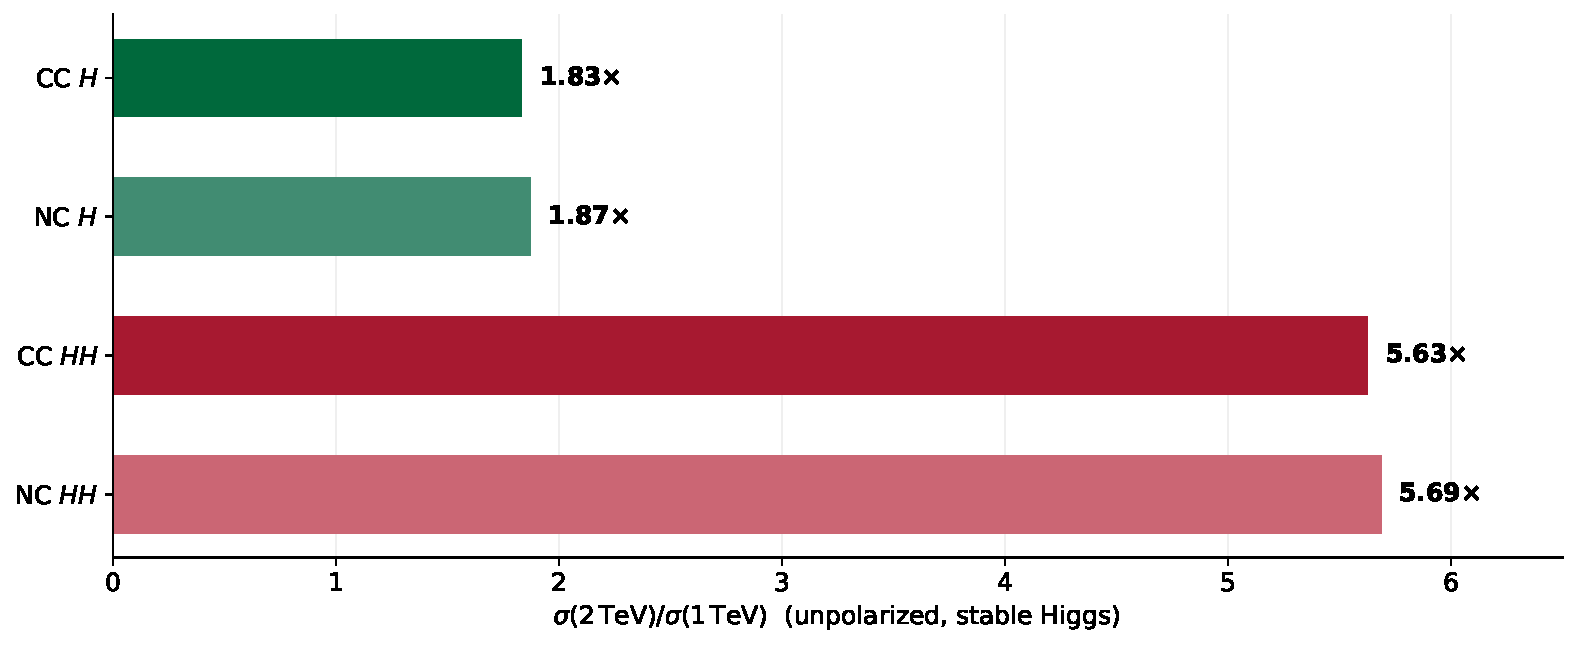
\includegraphics[width=\linewidth,height=0.52\textheight,keepaspectratio]{figures/Figure_energy_scaling.pdf}
\end{center}


\column{0.45\textwidth}
\begin{block}{Hypothetical $\mathcal L=3$ ab$^{-1}$}
\justifying 
At $P_{\mu^+}=80\%$:\\[.3em]
CC $HH$, 1 TeV: $\sim400$ produced events.\\[.3em]
CC $HH$, 2 TeV: $\sim2263$ produced events.\\[.3em]
NC $HH$, 2 TeV: $\sim193$ produced events.
\end{block}
\end{columns}

\key{\justifying These are raw inclusive yields: \emph{before} Higgs decays, tagging, acceptance, backgrounds or realistic luminosity allocation.}

%\src{Ratios derived from unpolarized 48-run CSV; $3$ ab$^{-1}$ is illustrative, not a machine forecast.}
\end{frame}




\part{Fiducial four-bottom portfolio}
\section{Fiducial four-bottom portfolio}







% Slide 27 / CC Double Higgs to $4b$ and Complete $\nu\bar\nu4b$
\begin{frame}[t]{CC Double Higgs to $4b$ and Complete $\nu\bar\nu4b$}
\small

\begin{columns}%%%[T,onlytextwidth]
\column{0.50\textwidth}
\begin{block}{FCC-$\mu e$}
\[\mu^+e^-\to\nu_e\bar\nu_\mu HH\to\nu_e\bar\nu_\mu4b\]
\[\mu^+e^-\to\nu_e\bar\nu_\mu b\bar bb\bar b\]
Machine-like $\sqrt{s}=0.980,1.913$ TeV.
\end{block}
\column{0.5\textwidth}
\begin{block}{Muon collider}
\[\mu^+\mu^-\to\nu_\ell\bar\nu_\ell HH\to\nu_\ell\bar\nu_\ell4b\]
\[\mu^+\mu^-\to\nu_\ell\bar\nu_\ell4b\]
$\ell=e,\mu,\tau$ (summed). $\sqrt{s}=1,2$ TeV.
\end{block}
\end{columns}
\key{Resonant $HH$ samples are distinct from the full $4b$ matrix element, which already contains Higgs and continuum contributions.}

%\src{October 2026 CC HH4b process inventory and audited CERN runs.}
\end{frame}








% Slide 28 / Four-Bottom Reconstruction and Fiducial Selection
\begin{frame}[t]{Four-Bottom Reconstruction and Fiducial Selection}
\small

\begin{block}{Charged-current $HH\to4b$ and full $\nu\bar\nu4b$}
\begin{center}
\large
$|\eta_{b_i}|<5\quad(i=1,\dots,4),\qquad p_{T,b}^{\min}=0$\\[.7em]
$110<m_{b\bar b}^{(1)}<130\,\mathrm{GeV},\qquad 110<m_{b\bar b}^{(2)}<130\,\mathrm{GeV}$
\end{center}
\end{block}
\begin{itemize}
\justifying 
\item Two disjoint $b\bar b$ pairs; source implementation uses allowed charge-opposite pairing assignments.
\item Observables defined using \emph{partons}, not clustered jets: no shower, tagging or detector effects.
\item NC samples additionally regulate the outgoing charged leptons with $p_{T,\ell}>1$ GeV at generation.
\item The later $\mu^+\mu^-\to ZH\to4b$ study uses 80-130 GeV windows instead.
\end{itemize}

%\src{CC four-bottom audit; NC three-process audit; 29 October ZH report.}
\end{frame}





% Slide 29 / Fiducial CC $HH$ and $4b$: FCC-$\mu e$ vs Muon Collider
\begin{frame}[t]{Fiducial CC $HH$ and $4b$: FCC-$\mu e$ vs Muon Collider}
\small

\begin{block}{LO parton-level fiducial cross sections [fb]}
\begin{center}\scriptsize\setlength{\tabcolsep}{5pt}\renewcommand{\arraystretch}{1.35}
\begin{tabular}{lcll}\toprule
Collider & $\sqrt{s}$ & $HH\to4b$: P0 / P80 & Complete $\nu\bar\nu4b$: P0 / P80\\\midrule
FCC-$\mu e$ & 0.980 TeV & 0.04912 / 0.08816 & 0.05355 / 0.09195\\
$\mu^+\mu^-$ & 1.000 TeV & 0.07047 / 0.11582 & 0.07530 / 0.12472\\
FCC-$\mu e$ & 1.913 TeV & 0.26478 / 0.47611 & 0.28157 / 0.50745\\
$\mu^+\mu^-$ & 2.000 TeV & 0.30624 / 0.54606 & 0.32480 / 0.57873\\\bottomrule
\end{tabular}\end{center}
\end{block}

\begin{alertblock}{Interpretation requires consistent normalisation}
Earlier resonant $HH\to4b$ used $\mathrm{BR}(H\to b\bar b)=0.844640$; these historical fiducial rates should not be treated as conventional precision-SM $4b$ yields.
\end{alertblock}

%\src{Historical CERN CC HH4b review package; $|\eta\_b|<5$, two 110--130 GeV pairs.}
\end{frame}






% Slide 30 / Resonant $HH$, Nonresonant $4b$ and Interference
\begin{frame}[t]{Resonant $HH$, Nonresonant $4b$ and Interference}
\small

\begin{center}\large
$\mathcal M_{\rm full\,4b}=\mathcal M_{HH}+\mathcal M_{\rm single\,H}+\mathcal M_{\rm nonres}+\cdots$
\end{center}
\begin{columns}%%%[T,onlytextwidth]
\column{0.5\textwidth}
\begin{block}{Different generator objects}
\begin{itemize}
\justifying 
\item Resonant $HH$ decay chains impose intermediate resonances.
\item Full $\nu\bar\nu4b$ includes allowed trees and interference.
\item Single-resonant and continuum pieces can overlap.
\end{itemize}\end{block}
\column{0.5\textwidth}
\begin{alertblock}{Danger of naive subtraction}
\justifying 
$\sigma_{\rm full}-\sigma_{HH}$ is \emph{not} generically an independently simulated, gauge-invariant physical background: interference, off-shellness, generator settings and resonance definitions matter.
\end{alertblock}
\end{columns}
\key{Next step: common-generation comparison with resonance-aware integration and detector-driven regions.}

%\src{CERN CC HH4b process cards and 1 TeV audit; general amplitude-coherence principle.}
\end{frame}





% Slide 31 / Neutral-Current Four-Bottom Channel Definitions
\begin{frame}[t]{Neutral-Current Four-Bottom Channel Definitions}
\small

\begin{block}{Distinct NC generator samples at $\sqrt{s}\simeq0.980$ TeV}
\begin{enumerate}
\justifying 
\item $e^-\mu^+\to e^-\mu^+HH\to e^-\mu^+4b$ (double Higgs).
\item $e^-\mu^+\to e^-\mu^+b\bar b H\to e^-\mu^+4b$ (associated Higgs).
\item $e^-\mu^+\to e^-\mu^+b\bar b b\bar b$ (complete final-state amplitude).
\item Same $4b$ final state with internal Higgs graphs excluded (continuum diagnostic).
\end{enumerate}
\end{block}
\begin{itemize}
\justifying 
\item Outgoing-lepton generation cut: $p_{T,\ell}>1$ GeV.
\item Four $b$ partons with $|\eta_b|<5$ and two $110$--$130$ GeV pairs.
\item Samples are \emph{not} mutually exclusive event classes; graph exclusions are not automatically gauge invariant.
\end{itemize}

%\src{NC three-process archived validation (27 Oct); continuum diagnostic (28 Oct).}
\end{frame}





% Slide 32 / NC Four-Bottom Cross Sections and Their Limitations
\begin{frame}[t]{NC Four-Bottom Cross Sections and Their Limitations}
\small

\begin{center}\setlength{\tabcolsep}{7pt}
\begin{tabular}{lrr}\toprule
Process at $\sqrt{s}=0.980$ TeV & $\sigma_{\rm fid}$ [fb] & Comment\\\midrule
NC $HH\to4b$ & 0.0063824 & Resonant $HH$\\
NC $b\bar bH\to4b$ & 0.0129250 & Overlaps HH-sensitive phase space\\
Complete NC $4b$ & 0.0077129 & 442/30,000 events pass\\
H-excluded continuum & 0.0008253 & 88/50,000 pass\\\bottomrule
\end{tabular}\end{center}
\begin{alertblock}{Outstanding numerical consistency issue}
\justifying 
Full $4b$ fiducial rate ($0.00771$ fb) lies below the separately generated $b\bar bH$ rate ($0.01293$ fb): this is \textbf{not explained} by the archived audit. Do not attribute it to interference without validation.
\end{alertblock}
\key{\justifying Priority: resonance-aware integration, independent seeds and independent $4b$ pairing/replay.}

%\src{NC three-process audit 27 Oct 2026, pp. 1--2; continuum report 28 Oct.}
\end{frame}






% Slide 33 / Associated $b\bar bH$ at Higher Energy and Polarization
\begin{frame}[t]{Associated $b\bar bH$ at Higher Energy and Polarization}
\small

\begin{block}{Selected preliminary +80\% $\mu^+$ results}
\begin{center}\begin{tabular}{lcc}\toprule
Collider & $\sqrt{s}$ [TeV] & $\sigma_{\rm fid}$ [fb]\\\midrule
FCC-$\mu e$ & 1.913 & 0.081843\\
$\mu^+\mu^-$ & 2.000 & 0.094913\\\bottomrule
\end{tabular}\end{center}
\end{block}

\begin{itemize}
\justifying 
\item $b\bar bH\to4b$ with outgoing charged leptons; distinct from $\nu\bar\nu HH$.
\item Exact generator definitions, selection rules and available statistics must be aligned before precision comparison.
\item May contain singly and doubly Higgs-resonant regions, depending on the process definition.
\end{itemize}

\key{\justifying Associated-Higgs benchmarks are useful for background strategy, but these rates are \emph{preliminary}.}

%\src{FCCue\_MuC\_Polarized\_AssociatedHiggs\_Results\_20261028.pdf; source inventory.}
\end{frame}






% Slide 34 / Muon-Collider $ZH\to4b$: Distinct Four-Bottom Topology
\begin{frame}[t]{Muon-Collider $ZH\to4b$: Distinct Four-Bottom Topology}
\small

\begin{block}{Explicit MadGraph resonant decay chain}
\texttt{generate mu+ mu- > z h QCD=0 QED=2, z > b b\textasciitilde{}, h > b b\textasciitilde{}}
\end{block}
\begin{center}\begin{tabular}{lcc}\toprule
$\sqrt{s}$ & $\sigma_{\rm before}$ [fb] & $\sigma_{\rm fid}$ [fb]\\\midrule
1 TeV & 1.564500 & $1.527161\pm0.001589$\\
2 TeV & 0.378880 & $0.369294\pm0.000408$\\\bottomrule
\end{tabular}\end{center}
\begin{itemize}
\justifying 
\item Four $b$ partons, $|\eta_b|<5$, two pairs in 80-130 GeV; $p_T^{\min}(b)=0$.
\item Includes $Z\to b\bar b$ and $H\to b\bar b$ decays; no extra BR factors.
\item Ordinary $s$-channel $\mu^+\mu^-\to Z^*\to ZH$ has no $\mu^+e^-$ counterpart with flavour-conserving SM couplings.
\end{itemize}

%\src{Muon Collider ZH to 4b, 29 Oct 2026, revised 80--130 GeV selection.}
\end{frame}






% Slide 35 / What the Four-Bottom Programme Establishes
\begin{frame}[t]{What the Four-Bottom Programme Establishes}
\small

\begin{columns}%%%[T,onlytextwidth]
\column{0.5\textwidth}
\begin{exampleblock}{Reliable building blocks}
\begin{itemize}
\justifying 
\item Fiducial $HH\to4b$ cross sections.
\item Complete $\nu\bar\nu4b$ amplitude comparisons.
\item NC associated-Higgs and full $4b$ samples.
\item Resonant muon-collider $ZH\to4b$ reference.
\end{itemize}\end{exampleblock}
\column{0.5\textwidth}
\begin{alertblock}{Unresolved before sensitivities}
\begin{itemize}
\justifying
\item Earlier Higgs BR normalization.
\item NC full versus $b\bar bH$ rate inconsistency.
\item Physical acceptance of very forward particles.
\item Detector response and multijet backgrounds.
\item Independent seeds and NLO corrections.
\end{itemize}\end{alertblock}
\end{columns}

%\key{These are production-level benchmarks and a background-analysis starting point, not a validated $\lambda_3$ sensitivity forecast.}

%\src{October 2026 CERN analyses and independent QA notes.}
\end{frame}




\part{Higgs potential and research plan}
\section{Higgs potential and research plan}



% Slide 36 / Higgs Self-Couplings and the $\kappa_3$--$\kappa_{2V}$ Programme
\begin{frame}[t]{Higgs Self-Couplings and the $\kappa_3$--$\kappa_{2V}$ Programme}
\small

\begin{center}
$\displaystyle V(h)=\frac{m_h^2}{2}h^2+\frac{m_h^2}{2v}h^3+\frac{m_h^2}{8v^2}h^4$\\[.6em]
$\displaystyle \kappa_3=\frac{\lambda_3}{\lambda_3^{\rm SM}},\qquad \kappa_{2V}=\frac{g_{HHVV}}{g_{HHVV}^{\rm SM}}$
\end{center}
\begin{columns}%%%[T,onlytextwidth]
\column{0.5\textwidth}
\begin{block}{Why $HH$ constrains the potential}
\begin{itemize}
\justifying 
\item $VV\to H^*\to HH$ contains $\lambda_3$.
\item $HHVV$ contact and separate $HVV$ terms interfere.
\item At fixed other couplings: $\sigma(\kappa_3)=c_0+c_1\kappa_3+c_2\kappa_3^2$.
\end{itemize}\end{block}
\column{0.5\textwidth}
\begin{exampleblock}{Proposed scan}
\begin{itemize}
\justifying 
\item Common SM input, consistent HEFT/SMEFT model.
\item $\kappa_3$--$\kappa_{2V}$ grid at 1/2 TeV.
\item Charged and neutral currents, with polarization.
\end{itemize}\end{exampleblock}
\end{columns}

\key{No $\kappa_3$ or $\kappa_{2V}$ limit has yet been extracted from our 48 SM-rate calculations.}

%\src{Higgs potential (SM), original MG5 HH diagrams; future coupling work proposed.}
\end{frame}







% Slide 37 / Differential Observables, EFT and Parameter Degeneracies
\begin{frame}[t]{Differential Observables, EFT and Parameter Degeneracies}
\small

\begin{columns}%%%[T,onlytextwidth]
\column{0.5\textwidth}
\begin{block}{Observables to generate}
\begin{itemize}
\justifying 
\item $m_{HH}$, especially threshold versus high-mass tail.
\item $p_{T,H}$ and Higgs rapidities.
\item Higgs opening angle and $\cos\theta$.
\item Outgoing lepton $p_T,\eta$ in NC.
\item $\not{p}_T$ and $4b$ reconstruction for CC.
\end{itemize}\end{block}
\column{0.5\textwidth}
\begin{alertblock}{Interpretation strategy}
\begin{itemize}
\justifying 
\item HEFT: flexible Higgs-coupling modifiers.
\item SMEFT: gauge-invariant operator correlations, validity domain.
\item Joint CC+NC+FCC-ee inputs for coupling degeneracies.
\item Shape likelihood with realistic backgrounds.
\end{itemize}\end{alertblock}
\end{columns}

\key{The $HH$ threshold and high-$m_{HH}$ regions can respond differently to $\kappa_3$ and $\kappa_{2V}$.}

%\src{General EW VBF phenomenology; Cao et al., PRD 109 (2024) 073005.}
\end{frame}







% Slide 38 / Beyond Double Higgs: Triple-Higgs Production
\begin{frame}[t]{Beyond Double Higgs: Triple-Higgs Production}
\small

\begin{block}{Two proposed full SM MadGraph reactions (not yet executed)}
\texttt{generate e- mu+ > ve vm\textasciitilde{} h h h QCD=0}\\[.45em]
\texttt{generate e- mu+ > e- mu+ h h h QCD=0}
\end{block}
\begin{columns}%%[T,onlytextwidth]
\column{0.5\textwidth}
\begin{itemize}
\justifying 
\item Direct LO contributions involving $\lambda_4$, $\lambda_3$ and Higgs--gauge couplings.
\item Test $\sqrt{s}=1,2$ TeV at $P_{\mu^+}=0,80,100\%$.
\item Validate integration near $m_{HHH}\geq375$ GeV threshold.
\end{itemize}
\column{0.5\textwidth}
\begin{itemize}
\justifying 
\item Evaluate $\sigma_{HHH}\times\mathcal L$ before decay/cuts.
\item Explore $6b$, $4b2\tau$ and $4b2\gamma$ modes.
\item If rates are tiny, test higher-energy exploratory points separately.
\end{itemize}
\end{columns}

\key{No $HHH$ cross-section numbers or $\kappa_4$ sensitivities have been calculated; feasibility comes first.}

%\src{Proposed next-step calculations; not included in completed CERN runs.}
\end{frame}





% Slide 39 / Proposed Collaboration Work Packages
\begin{frame}[t]{Proposed Collaboration Work Packages}
\footnotesize

\begin{center}\setlength{\tabcolsep}{4pt}\renewcommand{\arraystretch}{1.03}
\begin{tabular}{p{2.25cm}p{6.0cm}p{2.5cm}}\toprule
Work package & Immediate deliverable & Discussion\\\midrule
WP1: baseline QA & common parameter cards, cut definitions, seed reruns & inputs / owners\\
WP2: Higgs EFT & tested $\kappa_3$--$\kappa_{2V}$ UFO/SMEFT framework & basis / validity\\
WP3: shapes & $m_{HH}$, $p_T$, angles, CC/NC polarization grids & observables\\
WP4: experiment & $HH\to4b$ decays, b tagging, NC lepton acceptance, backgrounds & detector scenario\\
WP5: triple Higgs & first SM $HHH$ cross sections and event-yield decision & feasibility\\
WP6: context & FCC-ee synergy, novelty vs earlier $e\mu$ HH literature & paper strategy\\\bottomrule
\end{tabular}\end{center}
\key{Workstream leadership and deadlines to be agreed by the four participants during this meeting.}

%\src{Proposed internal collaborative agenda; no responsibilities preassigned.}
\end{frame}





% Slide 40 / Summary: Results Established and Decisions for the Kick-off
\begin{frame}[t]{Summary: Results Established and Decisions for the Kick-off}
\footnotesize

\begin{columns}%%[T,onlytextwidth]
\column{.5\textwidth}
\begin{exampleblock}{Established preliminary results}
\begin{itemize}
\justifying 
\item 48 CC/NC $H/HH$ inclusive LO points.
\item CC $P_{\mu^+}=80\%$: $\sim1.8\times$ enhancement; NC $\sim1.175\times$.
\item $HH$ production grows $\sim5.6\times$ from 1 to 2 TeV.
\item Original MG5 $HHVV$, separate-emission and $H^*\to HH$ diagrams verified.
\item Fiducial $4b$ / $ZH$ comparisons available with caveats.
\end{itemize}\end{exampleblock}
\column{.47\textwidth}
\begin{alertblock}{Decisions requested}
\begin{enumerate}
\justifying 
\item Common machine/physics benchmarks?
\item Consistent Higgs branching fractions?
\item HEFT or SMEFT choice?
\item Priority $\kappa_3$--$\kappa_{2V}$ observables?
\item First detector/4b and $HHH$ tests?
\item Joint-paper scope and milestone?
\end{enumerate}\end{alertblock}
\end{columns}
\key{Can FCC-$\mu e$ deliver a \emph{distinctive combined} Higgs-coupling programme alongside FCC-ee?}

%\src{Synthesis of CERN LO studies (2026); future analysis and decisions explicitly proposed.}
\end{frame}








% --------------------------------------------------------------------------
% Thank You
% --------------------------------------------------------------------------
\begin{frame}[plain]
\begin{center}

\includegraphics[width=0.85\paperwidth,height=0.85\paperheight,keepaspectratio]{Thank_You_2.jpg}
\end{center}
\end{frame}

%=================================================================








\appendix

\part{Backup materials}
\section{Backup materials}




% Slide 41 / B1: FCC-$\mu e$ Machine Working Points (Proposal v2)
\begin{frame}[t]{B1: FCC-$\mu e$ Machine Working Points (Proposal v2)}
\small

\begin{block}{Proposal examples: 2 TeV $\mu^+$ beam (revised arXiv v2)}
\begin{center}\setlength{\tabcolsep}{6pt}
\begin{tabular}{lcc}\toprule
Quantity & $e^-$ at 45.6 GeV & $e^-$ at 120 GeV\\\midrule
$\sqrt{s}_{\mu e}$ & $\sim0.60$ TeV & $\sim0.98$ TeV\\
Peak $\mathcal L$ [$10^{34}\,\mathrm{cm}^{-2}\mathrm{s}^{-1}$] & 4.5 & 0.63\\
Collision rate [MHz] & 40 & 1\\
$\beta^*_{x,e^-}$ [m] & 0.24 & 0.08\\
$\beta^*_{y,e^-}$ [mm] & 3.5 & 2.3\\
$\mu^+$ bunch population [$10^{10}$] & 0.2 & 1.0\\\bottomrule
\end{tabular}\end{center}
\end{block}
\begin{itemize}
\justifying 
\item 5 TeV $\mu^+$ stage and standalone running are exploratory proposal options.
\item Design feasibility depends on source yield, emittance preservation, levelling and MDI.
\end{itemize}

%\src{Piotrzkowski arXiv:2610.40451v2, Table 1 p. 5; note different values in earlier version.}
\end{frame}





% Slide 42 / B2: Process Generator Syntax and Analysis Inventory
\begin{frame}[t]{B2: Process Generator Syntax and Analysis Inventory}
\small

\begin{block}{Exact inclusive MG5 commands}
\texttt{generate e- mu+ > ve vm\textasciitilde{} h QCD=0}\\
\texttt{generate e- mu+ > ve vm\textasciitilde{} h h QCD=0}\\
\texttt{generate e- mu+ > e- mu+ h QCD=0}\\
\texttt{generate e- mu+ > e- mu+ h h QCD=0}
\end{block}
\begin{block}{Other source-defined final states}
\scriptsize
FCC-$\mu e$: $\nu_e\bar\nu_\mu HH\to\nu_e\bar\nu_\mu4b$, full $\nu_e\bar\nu_\mu4b$; NC $e^-\mu^+HH\to e^-\mu^+4b$, $e^-\mu^+b\bar bH\to4b$, full NC $4b$ and Higgs-excluded diagnostic.\\
$\mu^+\mu^-$: $\nu_\ell\bar\nu_\ell HH\to\nu_\ell\bar\nu_\ell4b$, full $\nu_\ell\bar\nu_\ell4b$, $b\bar bH$, and $ZH\to4b$.
\end{block}

%\key{Exact historical generator restrictions and cuts are defined in original archives; do not infer unsupplied syntax.}

%\src{CERN 48-run process cards and October 2026 process inventory.}
\end{frame}






% Slide 43 / B3: Complete 1 TeV Inclusive Table with MC Errors
\begin{frame}[t]{B3: Complete 1 TeV Inclusive Table with MC Errors}
\scriptsize

\begin{center}\scriptsize $\sigma\pm\delta\sigma_{\rm MC}$ in fb, exact $\sqrt{s}=1$ TeV.\end{center}
\begin{center}\setlength{\tabcolsep}{3pt}\renewcommand{\arraystretch}{1.23}\begin{tabular}{rllll}\toprule $P_{\mu^+}$ & CC $H$ & CC $HH$ & NC $H$ & NC $HH$ \\ \midrule
0\% & $210.540\pm0.209$ & $0.074384\pm0.00013$ & $20.835\pm0.025$ & $0.0096201\pm0.0000146$ \\
20\% & $252.710\pm0.158$ & $0.088979\pm0.00015$ & $21.770\pm0.015$ & $0.010045\pm0.0000167$ \\
40\% & $294.730\pm0.271$ & $0.104016\pm0.00019$ & $22.660\pm0.014$ & $0.010487\pm0.0000160$ \\
60\% & $336.830\pm0.199$ & $0.118825\pm0.00021$ & $23.611\pm0.019$ & $0.010895\pm0.0000148$ \\
80\% & $378.570\pm0.243$ & $0.133230\pm0.00023$ & $24.476\pm0.015$ & $0.011308\pm0.0000174$ \\
100\% & $421.150\pm0.433$ & $0.148239\pm0.00024$ & $25.402\pm0.018$ & $0.011723\pm0.0000180$ \\
\bottomrule\end{tabular}
\end{center}
\vspace{-.4em}
\begin{block}{Source-validation fields}
\justifying	\scriptsize
24 unique entries; all status \texttt{COMPLETED\_UNVALIDATED}; each requests 30,000 events. Independent seeds and relative MC errors are in \texttt{data/cross\_sections\_48.csv}.\\[.15em]
\textbf{Seed convention:} source seeds are linked to the unique process/energy/polarization record; no common-seed substitution.
\end{block}

%\src{Original CERN review reports/cross\_sections.csv; all individual seeds in packaged CSV.}
\end{frame}





% Slide 44 / B4: Complete 2 TeV Inclusive Table with MC Errors
\begin{frame}[t]{B4: Complete 2 TeV Inclusive Table with MC Errors}
\scriptsize

\begin{center}\scriptsize $\sigma\pm\delta\sigma_{\rm MC}$ in fb, exact $\sqrt{s}=2$ TeV.\end{center}
\begin{center}\setlength{\tabcolsep}{3pt}\renewcommand{\arraystretch}{1.23}\begin{tabular}{rllll}\toprule $P_{\mu^+}$ & CC $H$ & CC $HH$ & NC $H$ & NC $HH$ \\ \midrule
0\% & $386.010\pm0.303$ & $0.418510\pm0.00066$ & $38.991\pm0.030$ & $0.054712\pm0.0000851$ \\
20\% & $463.490\pm0.399$ & $0.502952\pm0.00085$ & $40.760\pm0.027$ & $0.057089\pm0.0000871$ \\
40\% & $540.620\pm0.371$ & $0.587089\pm0.00100$ & $42.460\pm0.045$ & $0.059636\pm0.0000859$ \\
60\% & $617.270\pm0.428$ & $0.671917\pm0.00115$ & $44.171\pm0.042$ & $0.062066\pm0.0000868$ \\
80\% & $695.000\pm0.614$ & $0.754495\pm0.00128$ & $45.829\pm0.055$ & $0.064299\pm0.0000957$ \\
100\% & $772.690\pm0.517$ & $0.839521\pm0.00140$ & $47.642\pm0.033$ & $0.066770\pm0.00010$ \\
\bottomrule\end{tabular}
\end{center}
\vspace{-.4em}\begin{block}{Source-validation fields}
\justifying	\scriptsize
24 unique entries; all status \texttt{COMPLETED\_UNVALIDATED}; each requests 30,000 events. Original run IDs/seeds and errors are preserved in packaged CSV and CERN JSON.\\[.15em]
\textbf{Clarification:} this exact 2 TeV benchmark differs from historical FCC-$\mu e$ $\sqrt{s}=1.913$ TeV.
\end{block}

%\src{Original CERN review reports/cross\_sections.csv; all individual seeds in packaged CSV.}
\end{frame}






% Slide 45 / B5: Original MG5 Diagrams and Source Identification
\begin{frame}[t]{B5: Original MG5 Diagrams and Source Identification}
\scriptsize

\begin{columns}%%[T,onlytextwidth]
\column{.50\textwidth}
\centering\textbf{CC $H$ (1)}\\[-.2em]
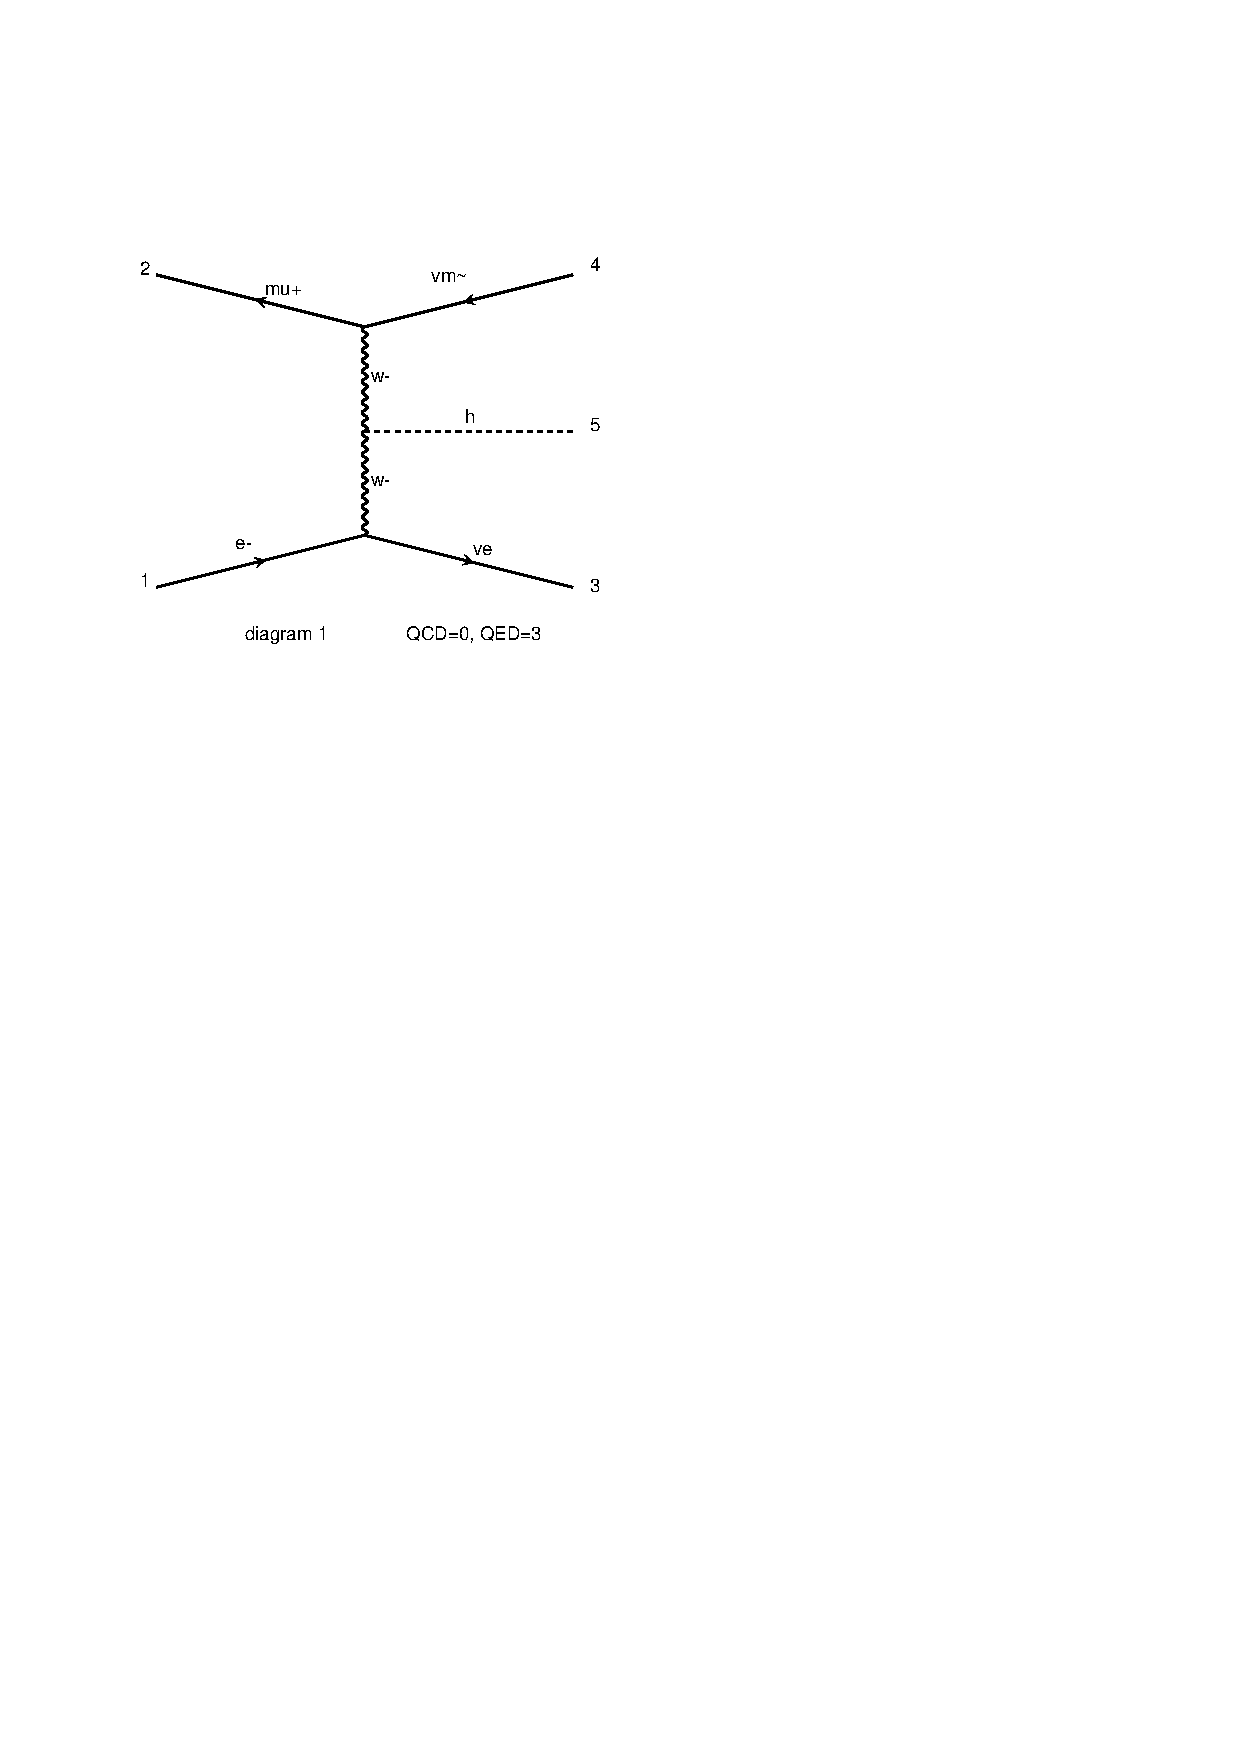
\includegraphics[width=.63\linewidth,height=.17\textheight,keepaspectratio]{figures/CC_H_diagrams_cropped.pdf}\\
\textbf{CC $HH$ (4)}\\[-.2em]
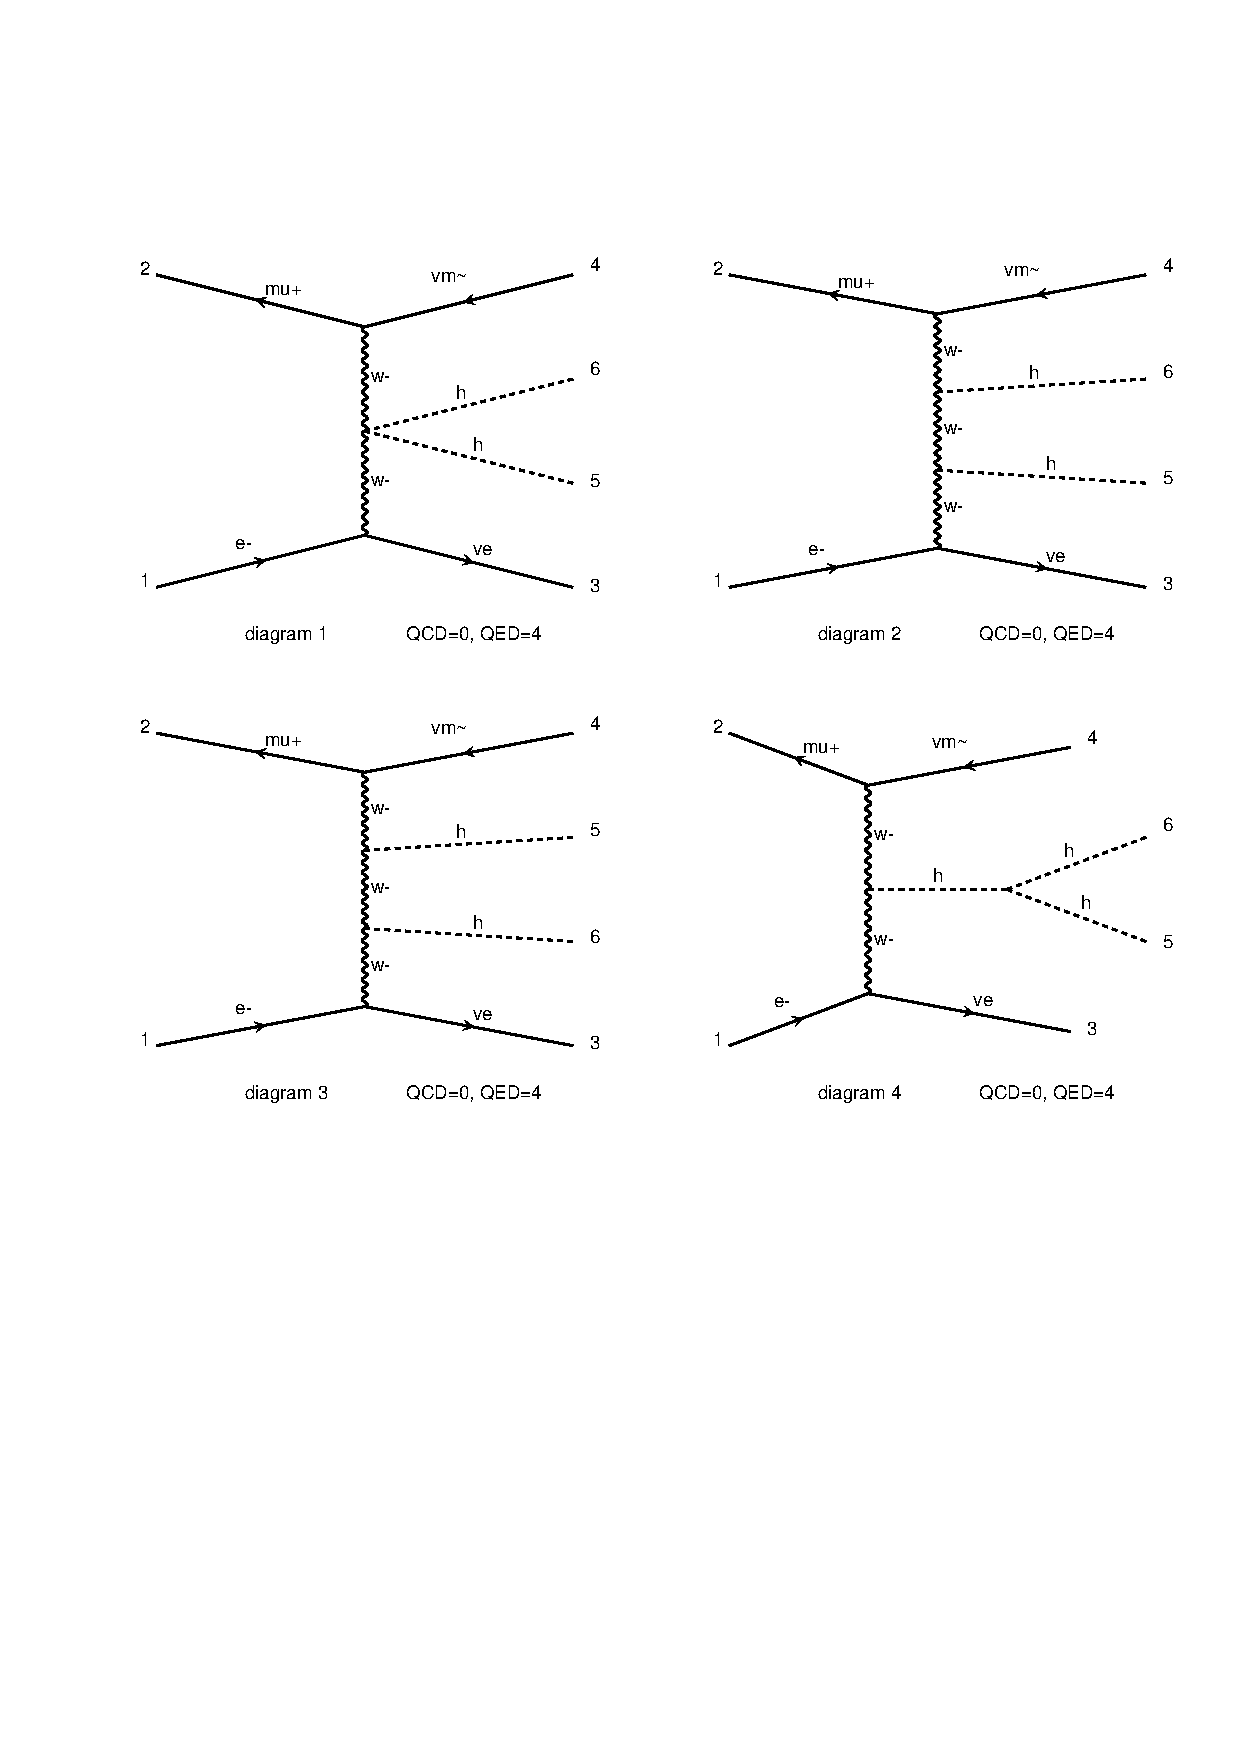
\includegraphics[width=.96\linewidth,height=.33\textheight,keepaspectratio]{figures/CC_HH_diagrams_cropped.pdf}
\column{.48\textwidth}
\centering\textbf{NC $H$ (1)}\\[-.2em]
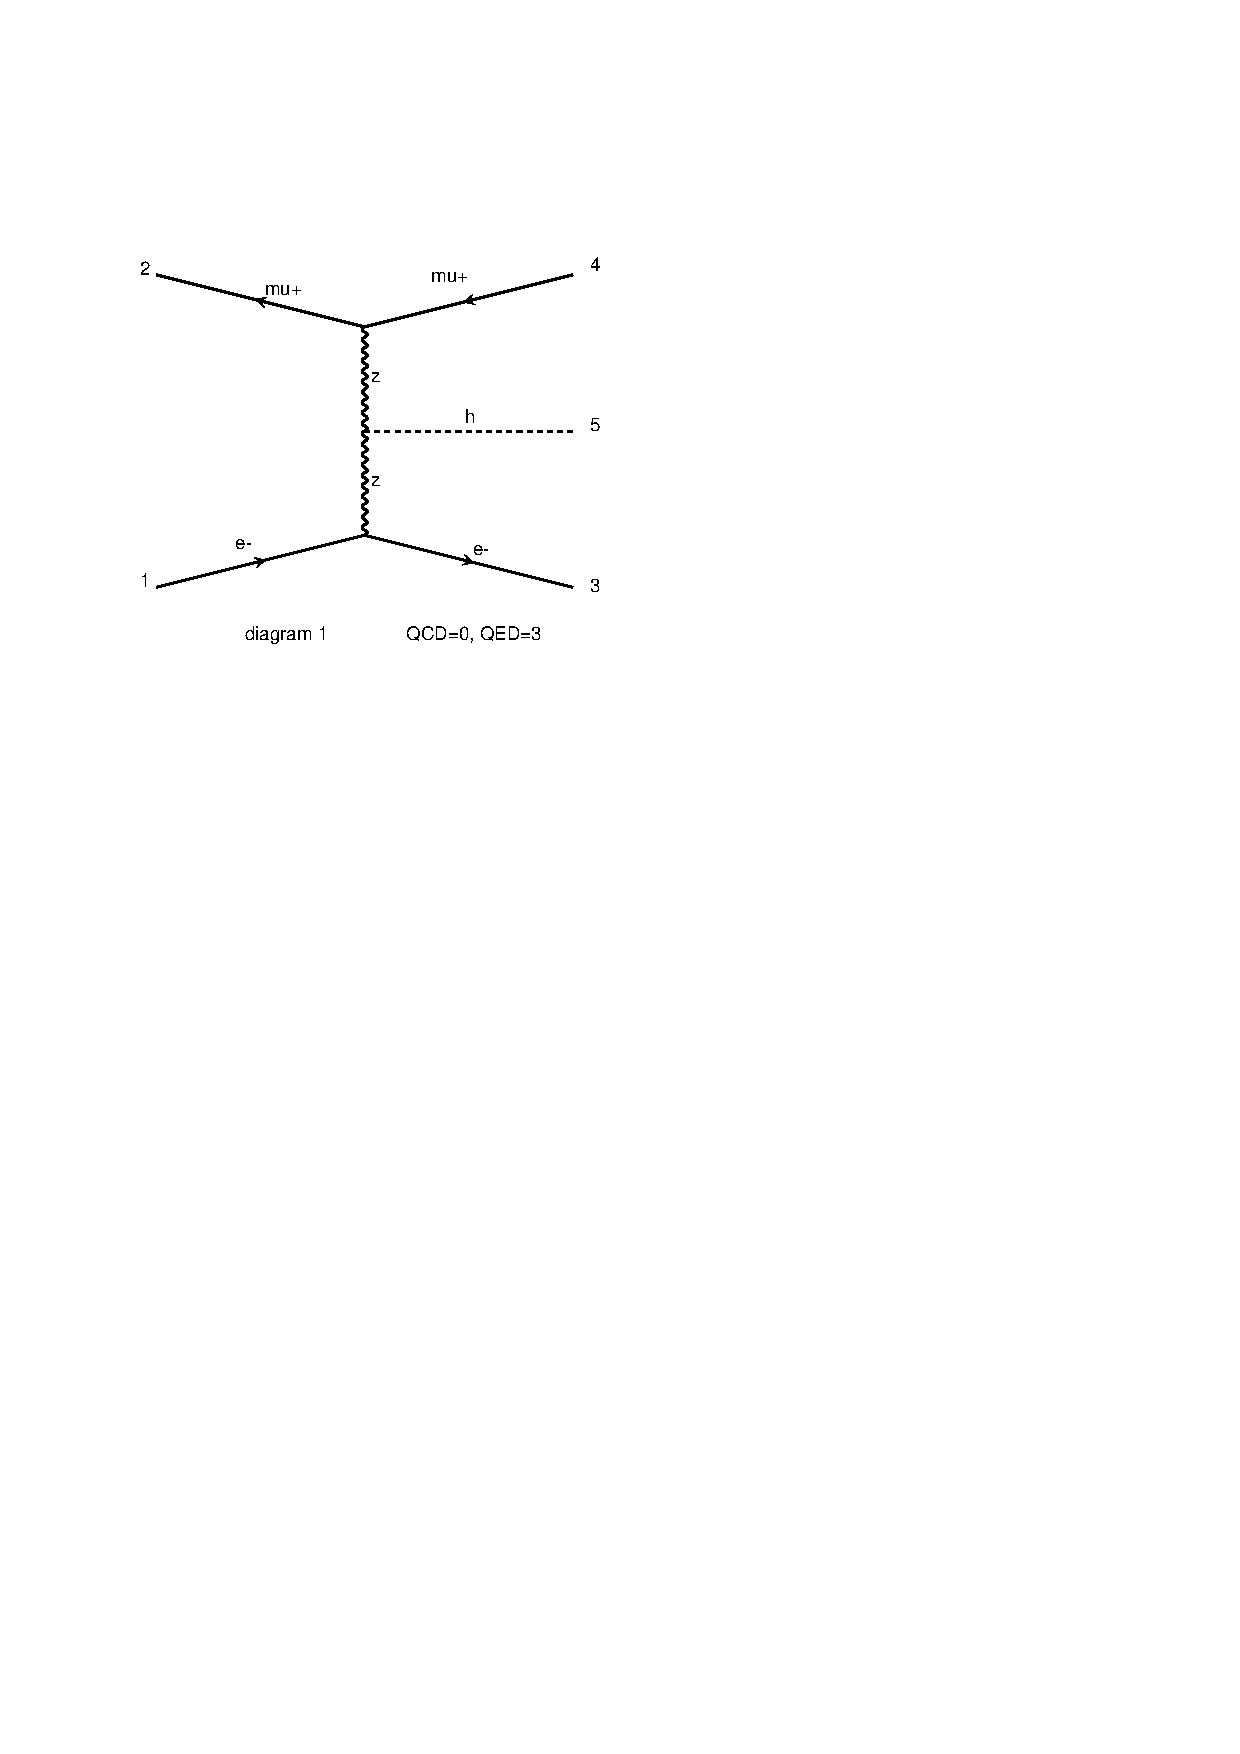
\includegraphics[width=.63\linewidth,height=.17\textheight,keepaspectratio]{figures/NC_H_diagrams_cropped.pdf}\\
\textbf{NC $HH$ (4)}\\[-.2em]
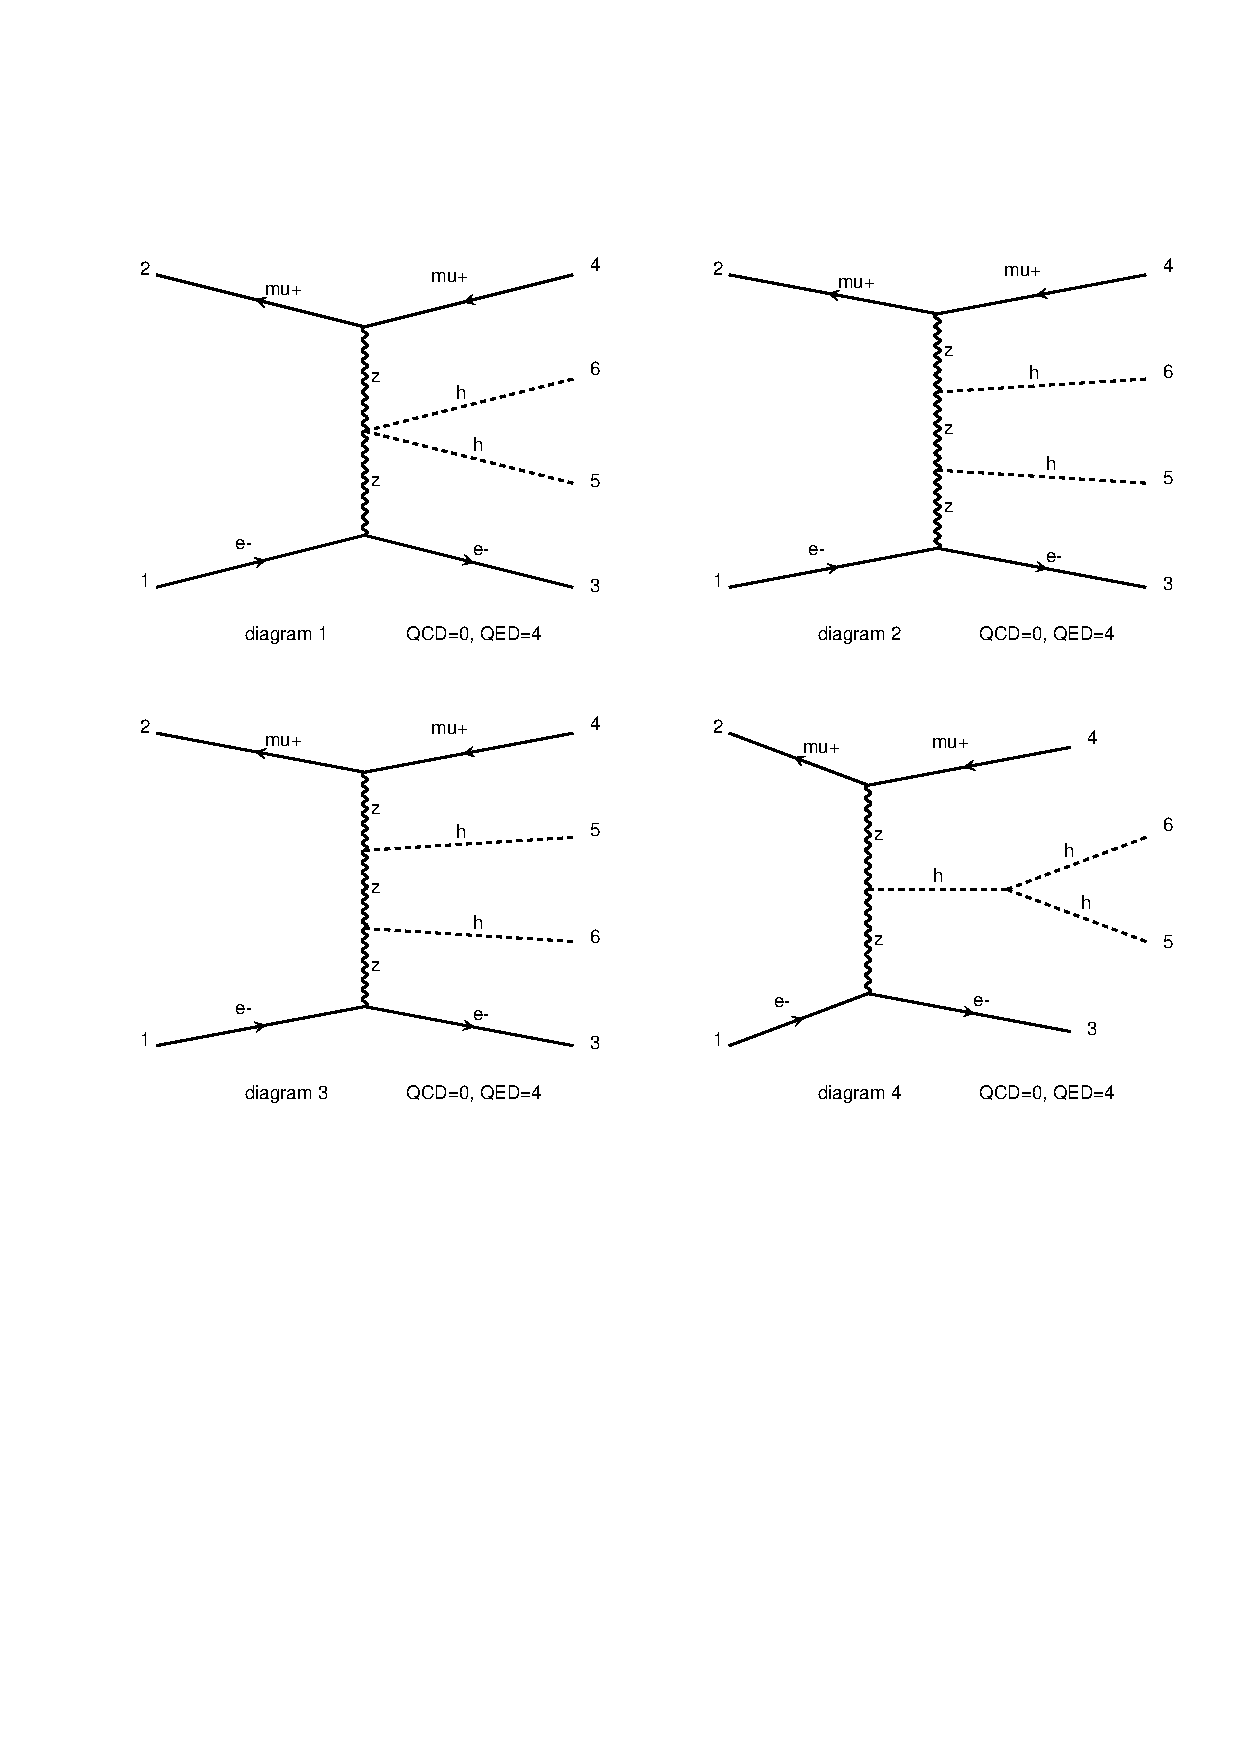
\includegraphics[width=.96\linewidth,height=.33\textheight,keepaspectratio]{figures/NC_HH_diagrams_cropped.pdf}
\end{columns}
\vspace{-.3em}\key{\justifying Original diagram numbers from MG exports retained. HH diagrams 1 contact; 2/3 separate emission; 4 virtual $H^*\to HH$.}

%\src{Original CERN MG5 matrix.pdf per process; vector crops for legibility.}
\end{frame}





% Slide 46 / B6: Fiducial Selection and Higgs-BR Normalization
\begin{frame}[t]{B6: Fiducial Selection and Higgs-BR Normalization}
\small

\begin{center}\setlength{\tabcolsep}{5pt}\renewcommand{\arraystretch}{1.23}
\begin{tabular}{p{3.0cm}p{3.6cm}p{4.2cm}}\toprule
Historical sample & Source cuts & Critical normalization / overlap\\\midrule
CC $HH\to4b$ / full $4b$ & $|\eta_b|<5$; two $110$--$130$ GeV pairs; $p_T^{\min}(b)=0$ & $\mathrm{BR}(H\to b\bar b)=0.844640$ for decays\\
NC $HH/b\bar bH$/full $4b$ & CC $b$ cuts + outgoing $p_{T,\ell}>1$ GeV generation & Overlapping amplitudes; full NC $4b$ still under review\\
Muon-collider $ZH\to4b$ & $|\eta_b|<5$; two $80$--$130$ GeV pairs; $p_T^{\min}(b)=0$ & $Z$ and $H$ branching already included in generator rate\\\bottomrule
\end{tabular}\end{center}

%\key{Do not equate generator-level partons with tagged jets; normalize common decay modes before projections.}

%\src{CC/NC 4b audits, 27--29 October 2026.}
\end{frame}






% Slide 47 / B7: Reproducibility, Integration and Open QA Checks
\begin{frame}[t]{B7: Reproducibility, Integration and Open QA Checks}
\footnotesize

\begin{columns}%%[T,onlytextwidth]
\column{0.50\textwidth}
\begin{exampleblock}{Verified in archives}
\begin{itemize}
\justifying
\item 48 unique rows: 4 channels $\times$ 2 $\sqrt{s}$ $\times$ 6 $P$.
\item All returned jobs recorded with success artifacts.
\item MG5 beam 1/2 energies and $P$ auditable.
\item Original process cards and selected run cards preserved.
\item Original diagrams independently inspected.
\end{itemize}\end{exampleblock}
\column{0.5\textwidth}
\begin{alertblock}{Not independently validated}
\begin{itemize}
\justifying
\item Multiple random-seed consistency.
\item NC forward-lepton cut/regulator stability.
\item Full NC $4b$ versus $b\bar bH$ inconsistency.
\item Decay normalization across old packages.
\item Detector/beam-background and higher-order theory.
\end{itemize}\end{alertblock}
\end{columns}
\key{MC integration uncertainty is not the total theory or detector uncertainty.}

%\src{CERN review/quality\_checks.json, 48-run audit, NC three-process validation.}
\end{frame}






% Slide 48 / B8: Primary References and Scientific Context
\begin{frame}[t]{B8: Primary References and Scientific Context}
\scriptsize

\begin{thebibliography}{9}
\justifying 
\scriptsize
\bibitem{proposal} K. Piotrzkowski, \emph{FCC-$\mu e$: High Energy, High Luminosity Muon--Electron Collider \& Neutrino Factory at CERN}, arXiv:2610.40451v2 (2026).
\bibitem{fcc} FCC Collaboration, \emph{Future Circular Collider Feasibility Study Report, Vol. 1}, Eur. Phys. J. C \textbf{85}, 1468 (2025), doi:10.1140/epjc/s10052-025-15077-x.
\bibitem{cao} Q.-H. Cao, K. Cheng, Y. Liu and X.-R. Wang, \emph{Measuring $hhWW$ coupling at lepton colliders}, Phys. Rev. D \textbf{109}, 073005 (2024).
\bibitem{int} H. Khanpour, \emph{MG LO process, run-card, numerical and diagram audits}, October-November 2026.).
\bibitem{mg} J. Alwall et al., \emph{The automated computation of tree-level and next-to-leading-order differential cross sections}, JHEP \textbf{07}, 079 (2014), arXiv:1405.0301.
\end{thebibliography}

\key{\justifying Collider projection, literature sensitivity and original MG  numerical calculations are differentiated throughout this presentation.}

%\src{Paper metadata checked against arXiv, FCC study report and PRD page; internal sources distributed separately.}

\end{frame}



\end{document}
